\documentclass[a4paper,oneside,12pt]{book}

%----------------------------------------------------------------------------------------
%	README!
%   Welcome. It's worth having a read through this file
%   to set up the broad parameters, such as the name of
%   the degree, the school/department, the type of work
%   (dissertation/Final Year Project/report, etc. as well
%   as your own details.
%----------------------------------------------------------------------------------------

%----------------------------------------------------------------------------------------
%	COVER PAGE
%   The cover page is laid out in title/title.tex. You can choose a colour
%   or black and white logo
%----------------------------------------------------------------------------------------

%----------------------------------------------------------------------------------------
%	THESIS INFORMATION
%   Put title, author name, supervisor name, degree, type of work, school, department in here
%   It will be used for the title page and for the embedded PDF information
%----------------------------------------------------------------------------------------

\newcommand{\thesistitle}{Machine Learning to go \textit{nyoom}} % Your thesis title, this is used in the title and abstract
\newcommand{\thesissubtitle}{Using Machine Learning to evaluate rowing training and predict training outcomes or performances}
\newcommand{\degree}{BA(Mod) in Science in Computer Science} % Replace with your degree name, this is used in the title page and abstract
\newcommand{\typeofthesis}{Final Year Project} % dissertation, Final Year Project, report, etc.
\newcommand{\authorname}{Liam Junkermann} % Your name, this is used in the title page and PDF stuff
%% Do not put your Student ID in the document, as TCD will not publish
%% documents that contain both your name and your Student ID.
\newcommand{\supervisor}{Dr.~Lucy Hederman} % replace with the name of your supervisor
%\newcommand{\cosupervisor}{Dr Alex Lee} % replace with the name of your co-supervisor if you have one
\newcommand{\keywords}{Sports Science, Machine Learning, Data Analysis, Data Visualisation, Personalisation} % Replace with keywords for your thesis
\newcommand{\school}{\href{https://www.tcd.ie/scss/}{School of Statistics and Computer Science}} % Your school's name and URL, this is used in the title page

%% Comment out the next line if you don't want a department to appear
% \newcommand{\department}{\href{http://researchgroup.university.com}{Department Name}} % Your research group's name and URL, this is used in the title page


%% Language and font encodings
\usepackage[T1]{fontenc} 
\usepackage[utf8]{inputenc}
\usepackage[english]{babel}
\usepackage{lmodern}

%% Bibliographical stuff
% \usepackage[]{cite}
\usepackage[backend=biber,style=ieee,maxcitenames=2,mincitenames=1]{biblatex}
%% Document size
% include showframe as an option if you want to see the boxes
\usepackage[a4paper,top=2.54cm,bottom=2.54cm,left=2.54cm,right=2.54cm,headheight=16pt]{geometry}
\setlength{\marginparwidth}{2cm}
%% Useful packages
\usepackage{amsmath}
\usepackage[autostyle=true]{csquotes} % Required to generate language-dependent quotes in the bibliography
\usepackage[pdftex]{graphicx}
\usepackage[colorinlistoftodos]{todonotes}
\usepackage[colorlinks=true, allcolors=black]{hyperref}
\usepackage{hyperxmp}
\usepackage{caption} % if no caption, no colon
\usepackage{sfmath} %use sans-serif in the maths sections too
\usepackage[parfill]{parskip}    % Begin paragraphs with an empty line rather than an indent
\usepackage{setspace} % to permit one-and-a-half or double spacing
\usepackage{enumerate} % fancy enumerations like (i) (ii) or (a) (b) and suchlike
\usepackage{booktabs} % To thicken table lines
\usepackage{fancyhdr}
\usepackage{xcolor} % to get TCD colour on headings
\usepackage{rotating,floatpag}
\usepackage{wrapfig}
\usepackage{pdfpages}

\numberwithin{equation}{chapter} %HS edit for (chapter.equation)
\pagestyle{plain} % Embrace simplicity!

\definecolor{tcd_blue}{RGB}{5, 105, 185}

%% It's personal taste but...
%% Uncomment the following block if you want your name and ID at the top of
%% (almost) every page.

%\pagestyle{fancy}
%\fancyhf{} % sets both header and footer to nothing
%\renewcommand{\headrulewidth}{0pt}
%\cfoot{\thepage}
%\ifdefined\authorid
%\chead{\it \authorname\ (\authorid)}
%\else
%\chead{\it \authorname}
%\fi
%% End of block

%% It is good practise to make your font sans-serif to improve the accessibility of your document.  Comment out the following line to disable it (but you really should not)
\renewcommand{\familydefault}{\sfdefault} %use the sans-serif font as default

\newcommand{\maxHR}{$\textnormal{HR}_{\text{max}}$}
%% If you insist on not using sans-serif (please don't), consider using Palatino instead of the LaTeX standard
%\usepackage{mathpazo} % Use the Palatino font by default if you prefer it to Computer Modern


%% Format Chapter headings appropriately
\usepackage{titlesec}
% \titleformat{\chapter}[hang]{\normalfont\huge\bfseries\color{tcd_blue}}{\thechapter}{1cm}{}{}

\title{\thesistitle}
\author{\authorname}


\hypersetup{
   pdftitle=\thesistitle, % Set the PDF's title to your title
   pdfauthor=\authorname, % Set the PDF's author to your name
   pdfkeywords=\keywords, % Set the PDF's keywords to your keywords
   pdfsubject=\degree, % Set the PDF's keywords to your keywords
   pdfinfo={
     pdfsupervisor=\supervisor, % Set the PDF's supervisor to your supervisor
     %pdfcosupervisor=\cosupervisor, % Set the PDF's cosupervisor to your cosupervisor if using
   }
}

\addbibresource{bibs/my.bib}
\frontmatter
\begin{document}
\begin{titlepage}

\center % Center everything on the page

%% All the text parameters should be taken from the start of the main.tex file.
%% You should only alter stuff here if you want to change the layout

%----------------------------------------------------------------------------------------
%	LOGO SECTION
%----------------------------------------------------------------------------------------
%% Choose one of the following -- a colour or black-and-white logo


\includegraphics{title/Trinity_RGB_transparent_main.png}\\[1cm] 
%
\includegraphics[width=12cm]{title/black-stacked-trinity.jpg}\\[1cm] 

\Large \school\\[1.5cm] % Minor heading such as course title
\ifdefined\department
\large \department\\[1.5cm] % Minor heading such as course title
\fi

%----------------------------------------------------------------------------------------
%	TITLE SECTION
%----------------------------------------------------------------------------------------
\makeatletter
{ \huge \bfseries \thesistitle}\\[1.5cm] % Title of your document
 

%----------------------------------------------------------------------------------------
%	AUTHOR SECTION
%----------------------------------------------------------------------------------------

\ifdefined\authorid
\authorname\\ % Your name
\authorid\\[2cm] % Your Student ID
\else
\authorname\\[2cm] % Your name
\fi

%----------------------------------------------------------------------------------------
%	Supervisor SECTION
%----------------------------------------------------------------------------------------

Supervisor: \supervisor\\[2cm] % Their name
\ifdefined\cosupervisor
Cosupervisor: \cosupervisor\\[2cm] % Their name
\fi


%----------------------------------------------------------------------------------------
%	DATE SECTION
%----------------------------------------------------------------------------------------

{\large \today}\\[2cm] % Date, change the \today to a set date if you want to be precise

 
%----------------------------------------------------------------------------------------
%	TYPE OF THESIS SECTION
%----------------------------------------------------------------------------------------
\vfill
 A \typeofthesis\ submitted in partial fulfilment\\of the requirements for the degree of\\
\degree

\vfill % Fill the rest of the page with whitespace

\end{titlepage}
\pagenumbering{roman}

% \section*{\Huge{Declaration}}
\vspace{1cm}
I hereby declare that this \typeofthesis\ is entirely my own work and that it has not been submitted as an exercise for a degree at this or any other university.

\vspace{1cm}
I have read and I understand the plagiarism provisions in the General Regulations of the University Calendar for the current year, found at \url{http://www.tcd.ie/calendar}.
\vspace{1cm}

I have completed the Online Tutorial on avoiding plagiarism `Ready Steady Write', located at \url{http://tcd-ie.libguides.com/plagiarism/ready-steady-write}.
\vspace{1cm}

I consent / do not consent to the examiner retaining a copy of the thesis beyond the examining period, should they so wish (EU GDPR May 2018).
\vspace{1cm}

% I agree that this thesis will not be publicly available, but will be available to TCD staff and students in the University’s open access institutional repository on the Trinity domain only, subject to Irish Copyright Legislation and Trinity College Library conditions of use and acknowledgement.  \textbf{Please consult with your supervisor on this last item before agreeing, and delete if you do not consent}
% \vspace{3cm}

Signed:~\rule{5cm}{0.3pt}\hfill Date:~\rule{5cm}{0.3pt}

% % \chapter*{Abstract}
\thispagestyle{plain}
\begin{center}
  \vspace{3cm}
  \textbf{\Huge\thesistitle}

  \begin{minipage}{12cm}
    \begin{center}
      \thesissubtitle
    \end{center}
  \end{minipage}

  \vspace{1cm}

  \authorname, \degree

  University of Dublin, Trinity College, 2024

  Supervisor: \supervisor

  \vspace{2cm}
  \textbf{Abstract}
\end{center}


Modelling human performance has been a challenging task for many years. The complexity of human physiology and the variety of factors that can influence performance make it difficult to develop accurate models. Machine learning, specifically neural networks, have proven particularly promising in applications to predict human performance. This project explores the approaches to data collection, analysis, and machine learning to predict rowing training outcomes and performances. The project aims to use machine learning techniques to predict performance using rowing data and explore the use of high-quality data to predict athlete injury. 

The project collected data from rowers using a web application developed as part of the project. This application was used to collect data on training sessions by allowing participants to connect data sources already used to track training with the project. The data collected was then analysed to develop features for a model, and visualisations were produced as feedback for participants. Unfortunately, the data collected was insufficient to develop a model to predict performance. Instead, the project explored the use of machine learning to predict injuries in runners, noting the approach and its potential application to appropriately collected rowing data.

Keywords: \keywords
% \newpage
\onehalfspacing\raggedright %\raggedright turns off justification and hyphenation

\section*{\Huge{Acknowledgements}}
Thanks Everyone!

You should acknowledge any help that you have received (for example from technical staff), or input provided by, for example, a company.

People to thank:
\begin{itemize}
  \item Mama + Papa
  \item Lucy
  \item The Boys (Trinity Defects)
  \item Participants
  \item John Harmon
\end{itemize}

\tableofcontents
\listoffigures
\listoftables
\newpage
\section*{\Huge{Vocabulary}}
\begin{tabular}{lp{9cm}l}
  \textbf{Heart Rate Metrics} \\
  HRV & Heart Rate Variability \\
  HR & Heart Rate \\
  $\textnormal{HR}_{\text{max}}$ & Maximum Heart Rate \\
  \textbf{Training Zones} \\
  UT2 & Basic Oxygen Utilisation Training \\
  UT1 & Oxygen Utilization Training \\
  AT & Anaerobic Threshold Training \\
  TR & Oxygen Transport Training \\
  AN & Anaerobic Capacity Training \\
  LT & Lactate Threshold \\
  \textbf{General Training Terms} \\
  Stroke Rate & The number of strokes completed per minute (like cadence in cycling or running) \\
  Split & The standard split in rowing is time to complete 500m \\
  \textbf{Data Providers} \\
  Strava & An exercise tracking platform with social media features commonly used by endurance athletes. \\
  Concept2 & The manufacturer of the most commonly used rowing machines. They provide an API for data access for sessions completed on the machines. \\
  Polar & A manufacturer of heart rate monitors, GPS watches, and other fitness tracking devices. \\
  Garmin & A manufacturer of heart rate monitors, GPS watches, and other fitness tracking devices. \\
% A&Area of the wing&$m^{2}$\\
% B\\
% C& Roman letters first, with capitals\ldots\\
% a&then lower case.\\
% b\\
% c\\
% $\Gamma$&Followed by Greek capitals\ldots\\
% $\alpha$&then lower case greek symbols.\\
% $\beta$\\
% $\epsilon$\\
% TLA&Finally, three letter acronyms and other abbreviations arranged alphabetically\\
\end{tabular}
\vspace{2cm}

% If a parameter has a typical unit that is used throughout your report, then it should be included here on the right hand side.

% If you have a very mathematical report, then you may wish to divide the nomenclature list into functions and variables, and then sub- and super-scripts.

% If you have a large number of acronyms, check out \href{https://www.overleaf.com/learn/latex/Glossaries} to make that more robust.

% Note that Roman mathematical symbols are typically in a serif font in italics.

\mainmatter
% maintaining separate .tex files for each chapter is good practice
\chapter{\label{ch:intro}Introduction}
This project explores the use of Machine Learning to model and predict rowing training outcomes and performances. Developing models for human performance is a complex and challenging task, with many factors influencing the outcome of a training session or cycle, and a variety of factors can influence performance when it matters. As early as 1975, linear models for performance were explored with reasonable success. Since then, many models have been developed to predict performance, with the most recent models implementing machine learning techniques and algorithms for this purpose. The aim of this project is to use some of the these techniques which have been developed to predict performance using rowing data. This chapter will introduce the general approach and motivation for this project, the expected outcomes, and a structure for the remainder of the report.

\section{Motivations}
The idea for this project is fuelled by a personal passion for rowing and performance alongside an academic interest in data analysis and machine learning. As a competitive rower for the last 12 years, I have produced a huge amount of data. In the last three years, I have been tracking my training and recovery data continuously with several wearables. At the moment, I wear at least three heart rate monitors at all times. This allows capture much of the same information for different platforms. These different platforms provide me with different feedback, of varying value, on training, recovery, and readiness to train more. I have always been interested in the data I produce and how I can use it to improve my training habits to perform optimally and avoid illness and injury -- the largest deterrents to my athletic growth in recent years. 

Despite the amount of data I have been producing, I have yet to consistently analyse it to provide feedback on my training. I am motivated by the prospect of developing a more effective approach to feedback, one that capitalizes on the wealth of data I have accumulated. By doing so, I hope to not only improve my performance but also contribute to the broader understanding of how data-driven approaches can be utilized in training prescription and personalisation.

This project was an opportunity to blend my love for rowing and sports science with my academic interest in data analysis and machine learning.  Ultimately driving for tangible improvements in training and performance, through the power of data analysis and machine learning.

% I love data, I love rowing, I want to use my data to row faster :)

\section{Goals}
There are several steps to this project, with the main goal being to develop a model which can predict rowing performance. This will be done by collecting data from rowers, performing initial analysis on this data to help develop features for a model, and then producing visualisations as feedback for participants. Finally, the primary goal of this project is to use this data to train a model which can predict performance, ideally predicting test scores, such as a 2km test on the rowing machine.

In developing a data collection method, the goal is to collect data from rowers in a way that is minimally invasive and requires no extra effort from participants (beyond some initial setup). It is notoriously difficult to collect data from athletes, especially those working or in college. As a result of the time-intensive nature of the sport, often athltes want solutions which require minimal setup, time and effort. The goal is to develop a system which could collect data without any extra effort from participants, and provide feedback on their training data.

For training feedback, the analysis must be relevant to rowers and visualisations effectively convey the analysis of their data without requiring an understanding of the underlying data analysis. The goal is to provide feedback on training data in a way that is easy to understand and actionable for participants.

The ultimate goal is to develop a model which could predict performance. This is the most ambitious goal of the project, due to the amount of data typically required to train a machine-learning model. This goal was adapted to explore the use of machine learning to predict injuries in runners.

\section{The Report}
The report begins in \hyperref[ch:background]{Chapter 2} with a review of the literature on rowing training and performance and the use of machine learning in sports science. This will provide the sports science-related knowledge necessary to understand the data collected and the approach used for analysis and model development. \hyperref[ch:data-collect-mng]{Chapter 3} discusses the approach used to collect and manage participant data, including the ethical considerations taken. Next, \hyperref[ch:data-anyl-viz]{Chapter 4} outlines the approach to developing a data analysis pipeline to provide participants with feedback on their training data. This will cover steps taken to clean and standardise the incoming data, the general approach which guided analysis, and how visualisations were developed and deployed. \hyperref[ch:ml]{Chapter 5} explores the machine learning approach taken. Unfortunately, due to limitations in data collection and time, the model was not able to be fully developed. However, the data collected and the initial analysis performed are discussed in this report. The machine learning goals were adapted to explore an approach to predict injuries in rowers, which is discussed in \hyperref[ch:ml]{Chapter 5}. The report concludes with a discussion of the results and potential future work in \hyperref[ch:discussion]{Chapter 6}.

\chapter{Background}
\label{chap:background}
This chapter will cover the basic background of rowing, the sports science which guides rowing training, and how an athletes body responds to training stimulus. Next, a review of performance modelling will explore the development of human performance modelling since the introduction of the basic Bannister model in 1975 \autocite{Bannister1976}. The section will outline how training load and performance can be quantified, and explain the way these approximations are used in various performance models to date.

\section{A brief introduction to rowing}
Rowing is an Olympic sport, raced across a 2,000 metre course, typically lasting six to seven minutes. It is classed as a power-endurance sport, this means training is focused on building aerobic, anerobic, and power while also developing rowing technique \autocite{Mäestu2005}. Most time is spent building endurance, next most time is spent building anerobic capacity, finally building strength and power through strength and condition sessions \autocite{Seiler2006}. The importance of power is more significant in rowing than in cycling given the relatively short duration of exertions, with longer distance racing typically only covering five to seven kilometers, or fifteen to twenty-five minutes. Conversely, road cycling, tends to last for a longer period of time, where the shortest races might last two hours. There are many different approaches to how training is conducted and which energy systems are targeted for improvements in efficiency or strength. This section will discuss the basic training principles which guide training, the way athletes respond to different kinds of training loads, and how performance is evaulated in rowing.

\subsection{Training Principles} \label{sub:training_principles}
Generally when a coach builds a training plan they have a few factors they can work with: volume, the amount of mileage or total time spent training, sessions intensity, how hard the given session is meant to be, and finally the frequency, or the time spent in different intensity zones. There are various ways to measure intensity, including heart rate, blood lactate concentration, velocity at maximal oxygen uptake (VO2 max), and relative perceived exertion (RPE) \autocite{Rosenblat2019}. 

\subsubsection{Training Zones}
Rowers tend to use heart rate zones or blood lactate concentration depending on access to the equipment to test blood lacate. Typically when a rower uses calculated aerobic zones each zone will be a percentage of \maxHR. Following this approach, zones are defined as follows:
\begin{description}
  \item[Z1] "Very Light" intensity, 50\% - 60\% of \maxHR
  \item[Z2] "Light" intensity, 60\%-70\% of \maxHR
  \item[Z3] "Moderate" intensity, 70\%-80\% of \maxHR
  \item[Z4] "Hard" intensity, 80\%-90\% of \maxHR
  \item[Z5] "Maximum" intensity, 90\%-100\% of \maxHR
\end{description}
The exact definition of these zones varies in the literature, as does the method to calculate \maxHR without a specific test. However, most high level athletes will have completed some kind of stress test to determine their \maxHR in order to train more effectively on their prescribed zones.
A rower who uses lactate based training zones might use the following zones:
\begin{description}
  \item[T1]  basic oxygen utilization training (UT2) [lactate~=~0-2 mmol/L]
  \item[T2]  oxygen utilization training (UT1) [lactate~=~2-3.5 mmol/L]
  \item[T3]  anaerobic threshold training (AT) [lactate~=~3.5-4.5 mmol/L]
  \item[T4]  oxygen transport training (TR) [lactate~=~4.5-6 mmol/L]
  \item[T5]  anaerobic capacity training (AN) [lactate $\geq$ 6 mmol/L] \autocite{Das2022}
\end{description}
Depending on how rigorous the testing protocol was, Heart Rate zones may be calculated for each zone, these may vary from the aerobic zones calculated from \maxHR.

The most basic zone approximation approach uses three zones based around certain physiological thresholds, like, lacate thresholds ($\textnormal{LT}_\text{1}$ and $\textnormal{LT}_\text{2}$) and ventilatory thresholds. Cyclists may use critical power to determine these three basic zones, although this practice has not become popular in rowing training. The zones become simply, low-intensity, moderate-intensity, and high-intensity. 

\subsubsection{Blood Lactate - A brief description}
Lactate is constantly produced by the body during the day. The concentration of blood lactate, measured in millimoles per litre (mmol/L), does not increase until the rate of lactate production surpasses the rate of lactate removal. Many things can affect the rate of lactate removal, training can improve the rate of lactate removal, with certain sessions targetting that adaptation. Blood lactate acts a biomarker used regularly to determine muscular fatigue during exercise. During a exercise lactate test a lactate profile is generated. Figure \ref{fig:lactateGraph} shows a chart showing two lactate profiles generated during two lactate tests about 14 weeks apart (98 days) in January and May of 2023. The test conducted saw the rower complete seven, four minute, efforts, at prescribed wattage targets. Details of each set of intervals can be found in \ref{sec:app-lactate-results}.
\begin{figure}
  \centering
  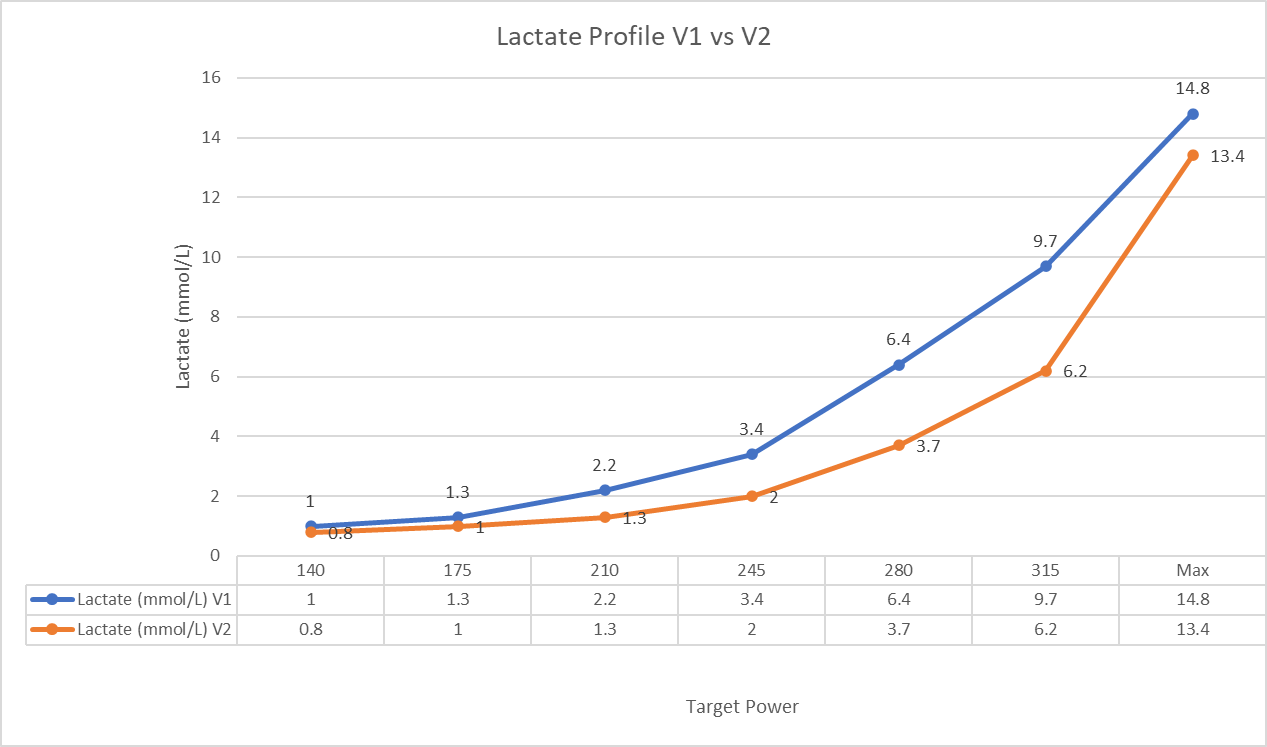
\includegraphics[width=\linewidth]{figures/lactateGraph.png}
  \caption[Lactate Profiles from January and May 2023]{Two lactate profiles completed 98 days apart following the protocol described above. Test one completed January 24, 2023. Test Two completed May 2, 2023}
  \label{fig:lactateGraph}
\end{figure}
These curves can be used to prescribe training as is described above.

\subsubsection{Training Prescription and Distribution}
There are a few different approaches for distributing intensity for endurance training. The three main methods are: polarised training, sweet spot or threshold training, and pyramidal training. This guides the final factor a coach considers when building a general training plan, frequency. For the purposes of comparing polarized training (POL), threshold training (THR), and pyramidal training (PYR), the more basic three zones of intensity will be used. The breakdown per zone for each training method is as follows:
\begin{description}
  \item[Polarised Training] Far more time spent in the low-intensity zone \autocite{Seiler2004}.

  \begin{description}
    \item[Low-Intensity] 75\%-85\% of total training volume
    \item[Medium-Intensity] 5\%-10\% of total training volume
    \item[High-Intensity] 5\%-10\% of total training volume  
  \end{description} 
  \item[Threshold Training] More time spent in the medium-intensity zone \autocite{Seiler2004}.

  \begin{description}
    \item[Low-Intensity] 45\%-55\% of total training volume
    \item[Medium-Intensity] 35\%-55\% of total training volume
    \item[High-Intensity] 15\%-20\% of total training volume  
  \end{description}
  \item[Pyramidal Training] Most time spent in low-intensity zone with progressively less time spent in higher zones \autocite{Selles2019}.

  \begin{description}
    \item[Low-Intensity] 75\%-85\% of total training volume
    \item[Medium-Intensity] 15\%-20\% of total training volume
    \item[High-Intensity] 5\%-10\% of total training volume  
  \end{description}
\end{description}

This report will not compare the effectiveness of different training distributions. Different distributions tend to be used by different sports, or depending on which energy system is being targeted. The use of polarized training is most common in rowing \autocite{Rosenblat2019}, although other training approaches have been used, especially around competition time.


\subsection{Energy Systems}
\label{sub:energy_systems}
In the human body there are two major types of skeletal muscle fibres, fast twitch, and slow twitch. Slow twitch muscles are used for longer, slower contractions where relative strength is low. Conversely, fast twitch muscles are shorter, faster contractions where strength is relatively higher. These types of fibres store energy differently and respond to training differently. Slow twitch muscles can be adapted to longer, lower effort, sessions and become resistant to fatigue, while fast twitch muscles fatigue easily, due to their lower glycogen capacity. Slow twitch muscle fibres have a low anaerobic capacity, while fast twitch muscle fibres have high anerobic capacities. These two kinds of fibres draw on two different energy systems: anaerobic and aerobic systems. These systems provide muscles with Adenosine Triphosphate (ATP) which is used by the mitochondria in the muscle fibre cells to produce energy, allowing the muscles to contract \cite{Göktepe2007}. 

The anaerobic system is used to provide energy to muscles to produce power without the use of oxygen. The anaerobic system typically provides energy for shorter periods of time. An immediate energy system can provide energy for 1-2 seconds of maximal work, this is typically used for resistance based strength training. More commonly in rowers, the short term energy system is used to provide energy to muscle fibres under significant strain. However, each time the energy system produces (ATP), lactate is also produced. This system is limited by an athletes ability to flush lactate from muscles. If the muscles are unable to flush the lactate quickly enough, the muscles will fatigue until failure forcing a stop to exercise. 

The aerobic, or long term energy, system is the slowest at providing energy to muscles. This system uses sugars, fats and oxygen to produce ATP. This system only works when large amounts of oxygen are available, which for rowers is typically during lower intensity sessions. Longer "steady state" sessions rely on the aerobic to provide energy to muscles, with these sessions also being used to build the aerobic system. By spending time in the appropriate training zones the aerobic system builds efficiency by creating new capillaries to support the slow twich fibres.

Rowers develop both their anaerobic and aerobic systems. Much of the winter season (typically September-March) is spent building the aerobic system, this is due to the longer length of any races done during this period, and to build a larger base on which to build a strong anerobic system. As the sprint racing season begins, or shortly before, more anerobic sessions will be introduced to build the system. Rowers will build their lactate tolerance, and spend more time at just-below-maximal efforts to prepare for the shorter race format.

% \subsection{Physiological Response to Training}
% Different people respond to training differently, for example, two people may be taking up a similar volume of oxygen (even $\textnormal{VO}_2$ utilization), but their muscles may be responding differently, producing different performances, or being able to sustain that load for different length of time. Differences in lactate threshold (LT), for example, can model the physiological state of an athlete during these efforts \autocite{Baldwin2000}. The goal for each training session is to, as efficiently as possible, become "fitter", in order to perform better. \textcite{Seiler2011} (2011) explored the effect of the use of different training intensities and durations on trained cyclists. 4x8min interval sessions yielded the most "\textit{pain for the gain}". Given that 

\subsection{Training Considerations}
When building a training plan many things are considered. Plans are typically built in macro-, meso-, and micro-cycles \cite{periodisation}. The macro-cycle in rowing will normally work on a yearly basis, with the overall target of performing at championship event at the end of the training year. 

Meso-cycles are typically seasonal or monthly cycles. For example, the autumn season is focused on building base fitness and forming a squad's technical style, there may be small races which a squad may attend, but any specific preparation for these events is unlikely. The winter months will be focussed on building the aerobic base, with some race preparation towards the end of the season being introduced. The spring season will see the first race events. Typically these are "Head races", longer races (5-6km) allowing the longer length, lower inensity sessions from the winter to be leveraged. This season will also an increase in interval and sprint race preparation in anticipation of the summer months. The summer season is the primary racing season, with the macro-cycle peak in performance. This meso-cycle will see a reduction in lower intensity aerobic sessions and an increase in anerobic intensity work to build fast-twitch muscle performances and the necessary racing performances of the shorter events.

Within these meso-cycles, there are micro-cycles typically lasting 7-14 days. It is crucial that these cycles are "periodised" appropriately. Periodisation is the budgeting of load across micro-cycles, ensuring athletes are experiencing the appropriate increase in intensity, followed by an appropriate length recovery period.

A coach will develop a training plan at the start of a new year, with a general idea of each cycle, and make adjustments as necessary throughout the year. If a coach had access to a system which could model the individual training responses for each athlete, individualised plans could be generated for each athlete, allowing the entire squad to train, and perform, at their physiological maximum. 

\subsubsection{Overtraining and burnout}
Training for endurance sports puts a large amount of strain physically, and mentally on athletes. Endurance athletes are conditioned to consistently push their bodies, making it difficult to identify when overtraining has occurred. Spending too much time in hard training zones without providing enough time to rest and recover leads to overtraining. Overtraining can be diagnosed when a performance decrease, as a result of training fatigued, has not gone away within two weeks of relative rest \cite{kayser2004chronic}. Overtraining can manifest symptoms physically and emotionally. Athletes may become depressed, chronically fatigued, and lose their appetites before a drop in performance. Ensuring training plans are appropriately periodised (load is managed in sustainable cycles of intensity and rest), and with enough variety in sessions to avoid monotony can help avoid overtraining. Athlete stress management outside of training is also crucial to managing overtraining.

Overtraining can often lead to burnout. Burnout is when an athlete gives up a sport entirely. With many athletes attaching their self-esteem to success in their sport, they risk burning out. This is particularly problematic when an athlete may be suffering from overtraining, or underperformance \cite{gustafsson2007burnout}.

Managing both overtraining and burnout are important when training, and can be considered when building a model of performance. Recognising overtraining can potentially prevent a promising athlete from retiring from their sport. By developing individual performance models, it can be easier to recognise overtraining and adjustments can be made to help the athlete recover more quickly.

\subsubsection{Tapering}
The concept of a taper is common among endurance athletes. Training blocks tend to be quite exhausting and typically leave athletes in an "over-reaching" state, they are constantly in a fatigued state. This encourages physiological adaptations but also negatively impacts performance. A taper period sees an athlete reduce their training load ahead of a competition \cite{Lawton2023}. Timing of the taper is important as athletes want to strike a balance between losing too much training time, and consequently fitness, and not having a long enough taper, and therfore still experiencing some training induced fatigue. Different taper strategies can be used, but typically session volume decreases, rather than session count. Typically as part of a taper a very short period (2-3 days) of high-intensity, interval, sessions is completed. This is followed by a longer period of recovery, or relative rest, in order to induce a "super-compensation" effect. This effect is a result of the body continuing to recover beyond the original baseline of fitness in anticipation of another period of high-intensity interval sessions. This results in a minor performance boost \cite{Kanwetz2016}.


\subsection{Performance}
There are two primary ways to measure a performance in rowing. First, on the rowing machine, a 2,000 meter, 6,000 meter, or 30 minute at stroke rate 20 (30 r20) test is normally used, depending on when during the season the test is done. This can be used to determine a rower's fitness and can be used to track progress for an athlete. These sessions are typically maximum effort sessions with some degree of taper (typically 4-7 days maximum) to elicit a peak performance. On the water, times can also be used to judge an entire crew, with external factors like wind direction and intensity, current flow, and temperature considered. Some boats and squads may use on the water telemetry to quantify the impact and power output of each rower. On-the-water performances may not always be peak efforts depending on a squad's seasonal focus or an event's progression (e.g. a maximal effort will rarely make an appearance in the heat stage of a heat-semi-final progression). Ergometer scores tend to be considered the purest way of quantifying a rower's performance, however, a combination of approaches can be used to quantify on-the-water performance.

\subsection{Summary}
Rowing training is quite time consuming for athletes. Many rowers will learn much of what has been discussed in this section to make better decisions themselves, or understand why training is done in a given way. The focus for a majority of the training cycle is to build a strong aerobic base in order to allow for higher "peak", ideally coinciding with the peak event for a season of training. For international athletes this will be a yearly cycle targetting World Championships, which is part of a four-yearly cycle targetting the Olympics. For national level athletes, national championships are typically the target, with Henley Royal Regatta featuring as a season's target. Coaches will normally take into account season targets and rower proficiency and base fitness when generating training plans. The target of this project is to make it easier for coaches and more accessible for athletes who may be more independent. 

\section{A Review of Performance Modelling}
The first wide spread approach to modelling performance was developed by \textcite{Bannister1976} with the Banister Fitness - Fatigue model, and further refined by \textcite{Morton1990} when defining training impulse to determine fitness and fatigue. The use of machine learning, specifically artificial neural networks has since been introduced in approaches to model performance. In preparation for the 2000 Olympics in Sydney, \textcite{Edelmannnusser2002} successfully predicted Olympic performances within an error of 0.05 seconds across a total time of 2:12.64 (min:sec) for the 200m backstroke event. \textcite{Edelmannnusser2002} specifically consider the limitation of using a linear model, such as the model proposed by \textcite{Bannister1976}, on training adaptation and performance; adaptation to training is inherently a complex non-linear process. 

This section will review basic approaches to systems modelling, exploring metrics which are commonly used to guide models and some non-linear systems models which have been explored. 

\subsection{Quantifying Training Load (Fatigue)}
\subsubsection{Rate of Perceived Exertion (RPE)} \label{subsub:rpe}
Rate of perceived exertion (RPE) is a scale, originally introduced by Gunnar Borg, to measure an athlete's effort. The original scale ranged from 6-20, where 6 would be no exertion at all, and 20 is maximal effort. This scale ranges from 6-20 to correspond more easily with heart rate, as the scale is used beyond just athletic settings. Therefore another scale, ranging from 0-10, was developed by Borg as well for use with "extreme intensity of activity", this is the scale normally used in athletic studies. The second scale is called a Category-Ratio (CR) scale where the reference anchor is RPE CR10 of 10, meaning maximal effort/pain. Session RPE (sRPE), using CR10, can be used, in conjunction with duration to determine session load \cite{Williams2017} using the equation $\textnormal{Load} = \textnormal{sRPE} \times \textnormal{Duration}$.

\begin{figure}
  \begin{minipage}[c]{0.4\linewidth}
      \centering
      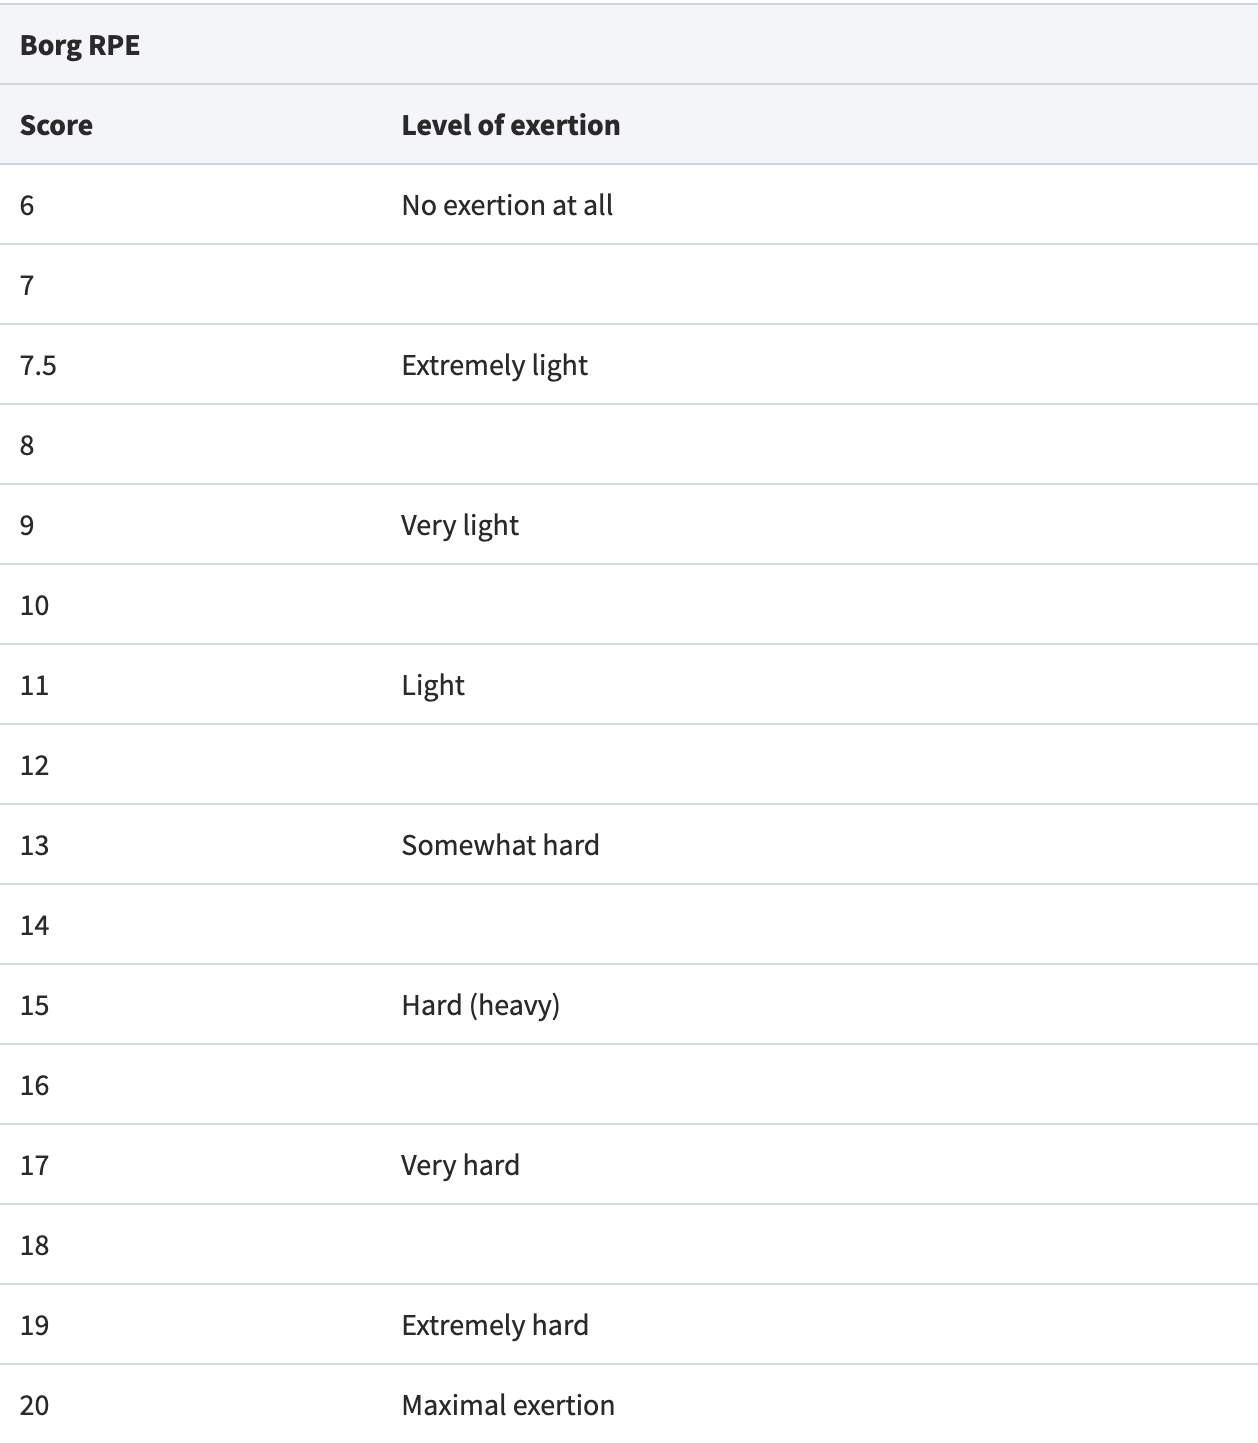
\includegraphics[width=\linewidth]{figures/borg20.png}
      \captionsetup{justification=centering}
      \caption[Borg 20]{The original Borg 6-20 RPE Scale \cite{Williams2017}} \label{fig:borg20}
  \end{minipage}\hfill
  \begin{minipage}[c]{0.4\linewidth}
      \centering
      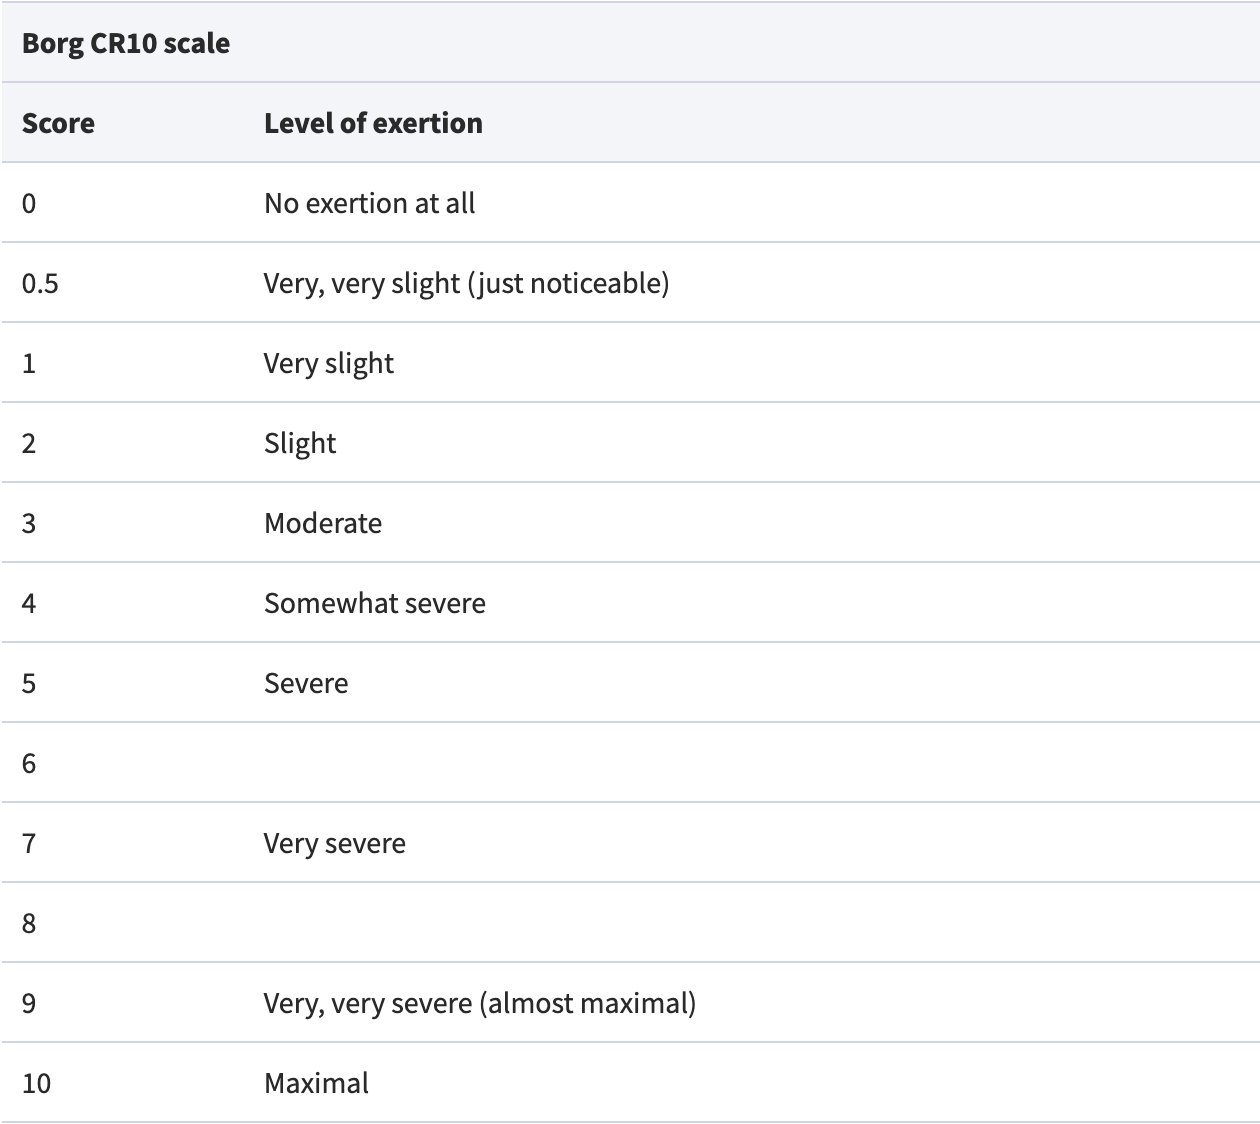
\includegraphics[width=\linewidth]{figures/borgc10.png}
      \captionsetup{justification=centering}
      \caption[Borg CR10]{The Borg Category-Ratio 10 RPE Scale \cite{Williams2017}}\label{fig:borgcr10}
  \end{minipage}
  \caption*{The two Borg RPE scales}
\end{figure}

\subsubsection{Training Impulse (TRIMP)}
Training Impulse (TRIMP) is a method to calculate training load and is defined as  $\textnormal{TRIMP} = \textnormal{Training Volume} \times \textnormal{Training Intensity}$ \autocite{TRIMPmethod}. There are many methods to calculate TRIMP, using different metrics to calculate training volume and training intensity. For the purposes of this project volume will simply be minutes, and intensity will be average heart rate (bpm), as the simplest TRIMP method outlined. Other modifications may apply a weighting against a heart rate metric to normalise longer sessions completed at a lower heart rate -- considering the noted difference in heart rate responses to training in male and female athletes \autocite{Morton1990}, alternatively, load can be calculated by using the product of RPE and duration (ie. $\textnormal{RPE} \times \textnormal{Duration (minutes)}$).

\subsubsection{Acute Chronic Workload Ratio (ACWR)}
Acute Chronic Workload Ratio (ACWR) can be used to monitor load in an athlete. It compares training load accumulated, in arbitrary units (AU), over the last seven days (acute workload) to the training load accumulated over the last twenty-eight days (chronic workload). The exact calculations used to determine acute and chronic workload depends on what type of ACWR model is selected. Additionally, the exact time periods considered for acute and chronic load can change depending on the application \cite{White2023}. Typically ACWR is used for injury management in team sports, but some articles have found it may not be effective for preventing injury as it is inaccurate way of approximating load \cite{Impellizzeri2020}. Training load estimation in rowing tends to be more objective given the objective internal load measurement of heart rate measured during a session. There is no clear consensus in literature about the effectiveness of using ACWR in injury prevention. As a relatively new concept, first published in 2016, more research into its efficacy and to provide validation needs to be completed \cite{Zouhal2021}. Regardless of its effectiveness in reducing injury, ACWR charts are easy to produce and provide easy feedback to rowers to see how training load can change week-to-week and ensuring load is not increased too quickly to begin to risk overtraining or injury.

\subsection{Impulse-Response Models} 
Impulse-response models are a group of models, built on the model initially introduced by \textcite{Bannister1976}. These models assume that a single exercise, or training session, produces two responses: fitness, or a positive performance response, and fatigue, or a negative performance response. A simplified version of this model is defined as 
\begin{equation}\label{eq:ffm}
  Performance = Fitness - Fatigue
\end{equation}
This simplified model is commonly called the Fitness-Fatigue impulse response model (FFM) and research since its initial introduction in 1975 has sought to refine how the $Fitness$ and $Fatigue$ components of this equation are defined.

\subsubsection{Banister Fitness-Fatigue Model}
 In the FFM model originally introduced in 1975 \cite{Bannister1976}, and built upon by \textcite{Morton1990} in 1990, the functions for fitness and fatigue were defined, considering a cumulative training load and a decay factor for each response. This decay factor is different for both the fitness and fatigue responses, resulting in a longer decay period for fitness than fatigue, but also differs from person to person, offering a parameter to be tuned for each athlete. First, a session needs to be quantified. A session is defined as:
\begin{equation}\label{eq:ban_imp_base}
  w(t) = D (\Delta \textnormal{HR ratio})
\end{equation}
where
\begin{equation*}
  \Delta \textnormal{HR ratio} = \frac{\textnormal{HR}_\textnormal{exercise} - \textnormal{HR}_\textnormal{rest}}{\textnormal{HR}_\textnormal{max} - \textnormal{HR}_\textnormal{rest}}
\end{equation*}
\textcite{Morton1990} acknowledged the disproportionate influence longer sessions at a low heart rate could have on resulting sessions $w(t)$, in arbitrary units (AU), so introduced a weighting factor $Y$. They determined $Y = e^{bx}$, where $b$ is a pre-selected value determined for men and women, and $x = \Delta \textnormal{HR ratio}$. So each training session is calculated as:
\begin{equation}\label{eq:ban_impulse}
  w(t) = D (\Delta \textnormal{HR ratio})Y
\end{equation}
Next, Fitness, $g(t)$, and Fatigue, $h(t)$, can be calculated. These two functions are defined as
\begin{equation}\label{eq:ban_fit}
  g(t) = g(t - 1)e^\frac{-i}{\tau_1} + w(t)
\end{equation}
and
\begin{equation}\label{eq:ban_fat}
  h(t) = h(t - 1)e^\frac{-i}{\tau_2} + w(t)
\end{equation}
where each function states the fitness and fatigue at the end of the day $t$, $i$ is the number of days between the training session being added and the last training session, and $\tau_1$ and $\tau_2$ are the decay time constants for fitness and fatigue respectively. Finally, to model performance, two more constants are introduced: $k_1$ and $k_2$. These constants are weighting factors for fitness and fatigue, they have "no direct physiological interpretation" \cite{Morton1990} but can be used to adjust the model for athletes who recover more quickly to heavy training load or require more time to recover from sessions across a taper period. Finally, performance is modelled as
\begin{equation}\label{eq:ban_perf}
  p(t) = k_1g(t)-k_2h(t)
\end{equation}
The model was originally developed using a swimmer. When evaluated using linear regression for the athlete-specific parameters ($\tau_1$, $\tau_2$, $k_1$, and $k_2$), the model reasonably estimates the performance outcome of a swimmer with relative confidence. No $r^2$ value is provided for the swimming application in 1975 \cite{Bannister1976}. In the 1990 model from \textcite{Morton1990}, two of the researchers participated in a training and testing regimen and a "good degree of fit" was observed, with $r^2$ values of 0.71 and 0.96 calculated for a slightly trained and an untrained runner respectively, with the former being given a starting 1000 AU points given some preexisting running fitness. The impulse-response model, if trained appropriately can help guide the structure and timing of a taper period for each athlete \cite{Morton1990}.
Versions of this kind of impulse-response model are used in basic analysis across many consumer fitness apps today, such as Training Peaks and Strava.

\subsubsection{Limitations to the Impulse-Response Model}
The Banister FFM simplifies human physiology quite effectively. However, in order to tune the parameters of the model, regular "criterion" testing needs to occur. These are maximal efforts done at regular intervals. During the testing of the \textcite{Morton1990} model refinements, both participants tested roughly once per week, something which is not feasible for high-level endurance athletes. This dependency on regular testing to tune parameters makes it particularly difficult to implement effectively as a holistic model for rowers. Furthermore, the use of data to adjust model parameters results in less data being available to model training behaviour.

The model only considers training load, specifically endurance training load, as an indicator for performance. Given the power dominance in rowing, a training block with seemingly less training load, as a result of more time and energy spent doing strength training, this can result in a bigger performance when tested next which may not be explained by changes in endurance training load. Additionally, the model does not consider other factors such as recovery and non-training strain an athlete might experience.

Finally, if the model is not constantly updated, it cannot predict future performances effectively. For the purposes of this project, a model would require an understanding of training behaviours in order to model the physiological response, predicting future performances. By modelling physiological response, suggestions can be made to improve certain energy system efficiency or effectiveness if needed. 

Impulse-response models are still widely used to model training and adaptation for athletes, their simplicity being a key factor for this. To more effectively model performances, without the need for constant testing, alternative models can and should be used. Impulse-response models can still be used in machine learning solutions, though, but as part of a larger ensemble approach \cite{Imbach2022}.

\subsection{Alternative Models}
There are models which employ more complicated mathematical approaches. This section will explore one of the most developed models, Performance Potential (PerPot), and explore artificial neural network approaches used by a number of researchers in recent years.

\subsubsection{Performance Potential (PerPot)}
Performance Potential (PerPot) was first introduced by \textcite{perl2001} in 2001. It is a performance potential meta-model which models responses to training input through a flow model. PerPot approaches performance modelling similarly to the impulse-response approach, each training load has an antagonistic response, two contradicting effects: response potential and strain potential. These can be compared to the impulse-response fitness and fatigue responses, respectively. Strain and response potentials impact the performance potential with differing decay factors, like impulse-response models as well. There have been reports of PerPot being effective in modelling cycling training \cite{Churchill2014}. PerPot, unfortunately, suffers from one of the key issues with impulse-response modelling: repeated testing is needed to tune the model's parameters. Additionally, due to the nature of the decay factors for strain and response potentials, the super-compensation effect is not considered with the basic PerPot model \cite{Churchill2014}. 

\subsubsection{Artificial Neural Network (ANN) approaches}
Artificial neural networks (ANN) have been used to effectively model performance based on training data as early as 2000 by \textcite{Edelmannnusser2002} where (200m - Backstroke) swimming performances at the 2000 Olympic Games were predicted based entirely on training data. In building their model, \textcite{Edelmannnusser2002} considered the use of linear models like the impulse-response model, but commented that biological adaptations are inherently non-linear, and therefore set out to "demonstrate that the adaptive behaviour of an elite female swimmer can be modelled by means of the non-linear mathematical method of artificial neural networks". 

Machine learning techniques require vast quantities of data in order to be effective. \textcite{Edelmannnusser2002}, however, used a single athlete, collecting 95 weeks of training data and 19 competitive performances. This is quite a small training set for a machine learning application. With only 19 performances to compare a performance model to, the risk of overfitting is significant. \textcite{Edelmannnusser2002} completed three data analysis steps to generate a model. The first two steps involved determining the impact of a 2-week taper period and the impact of a 2-week intense period immediately before the taper (3-4 weeks before competition) for steps one and two respectively. The final step combined the first two steps to determine the influence of the four weeks leading into competition. The result of this neural network approach was quite successful and \textcite{Edelmannnusser2002} concluded that neural networks can be effectively used on small datasets to predict performances. 

\textcite{Churchill2014} sought to build on the success of using ANNs by \textcite{Edelmannnusser2002} to model performance outcomes, but targeting professional cycling performances. Churchill, however, struggled to collect data for peak performances due to the strategic nature of cycling. Churchill did develop techniques to smooth noise in small datasets using an ensemble approach, citing the larger the number of neural networks used, the better smoothing was applied to noise. Artificial neural networks have consistently shown promise in predicting performances in swimming and cycling, even addressing small dataset issues which are prevalent in machine learning applications. This project aspires to build on these successes and apply ANN and ensemble techniques to individual rowing training data to predict ergometer performances.

\chapter{Data Collection and Management}
The first step in building any machine learning model is collecting, or acquiring, data with which to train and develop a model. To collect user data there were also ethical considerations to take into account and ethics approval was required. This chapter will discuss the data collection process, how the data was managed and stored for use in the project, and the ethical considerations and concerns that were a part of that data collection and storage development.

\section{Research Ethics Considerations and Approval}
When collecting data from participants, it is important to consider the ethical implications of that data collection. This is especially true when the data being collected is personal data, such as the data collected in this project. The data collected in this project was personal data, as it included information about the user's training sessions, including in many cases heart rate and GPS data, and their personal details such as their name and email address. As such, it was important to consider the ethical implications of collecting this data and to ensure that the data was collected in a way that was respectful of the user's privacy and rights. Furthermore, all of the participants are active competitors, many of them competing against the researcher in the same events. It was important to ensure that the data collected was not used in any way that could be seen as an unfair advantage. Some squads have strict policies surrounding the sharing of training data and scores; the same data privacy requirements were required to begin conversations with these squads and their members to collect data. 

When applying for ethics approval it was important to consider how user data could be protected both from unauthorised access and, in the unlikely event of a data leak, ensuring the exposure a user sees is minimal.

To ensure user data protection, much of the connection to an actual person is removed, the data is stored in a database with a unique identifier, and the user's email address is stored in a separate table. This means that if the database is accessed, the user's email address or other identifying information is not immediately available. The data is also stored in a secure database, with access restricted to only the researcher and the serverless functions used for analysis. To ensure data protection for participants during the project, all data received is encrypted at rest and in transit. A table linking the unique identifiers generated for each user and identifiable user data was stored securely on the researcher's personal machine making the de-pseudonymisation of the data more difficult. This key was kept to provide users feedback through the website and to allow the researcher to delete any collected information if a user elected to leave the project early.

There was some GPS data available in some training sessions submitted as part of the project. It was determined that this data, if leaked, would not be a significant risk to the user, as the data was only collected during on-the-water training sessions where many rowers train and compete normally. As most rowers in a squad train together, if the raw data for multiple sessions were leaked it would be nearly impossible to pinpoint which sessions belonged to which athletes given the number of total athletes training at any one time. 

Most of the analytics approaches were tested using the researcher's own training data. This ensured that the researcher did not get an unfair advantage when comparing to other athletes' data; any further analytics done for individual users was done using serverless functions meaning the researcher never had direct access to the raw data. These policies and procedures were included in the ethics application and were approved by the College Research Ethics Committee, and were shared with participants when in the recruitment stage. 

Following some difficulties with the new College Research Ethics Approval Management System (REAMS), an ethics approval application was submitted on November 2, 2023 and approval was granted on December 6, 2023. It is available in the appendix \ref{sec:ethics-approval-application}.

\section{Data Collection}
When developing the data collection pipeline, some key considerations were made. Firstly, the user effort per activity logged was to be as minimal as possible. Rowers typically have a lot of data to log, and the more effort required to log each activity, the less likely they are to do so. In many cases they were already logging their training elsewhere as a part of their squad's training program, therefore making the process of logging their sessions for this project as seamless as possible became a priority. Next, for what little interaction was required, the platform needed to be easy to use and intuitive. This was important as it reduced the workload of maintaining the platform, by responding to user queries, and encouraged users to continue using the platform due to its ease of use.

Considering the minimum requirements for a successful data collection pipeline, a website was developed to manage data provider connections and view training feedback. This website worked in conjunction with a series of serverless functions to automatically collect and analyse user sessions, and generate the feedback which was presented in the website.

\subsection{The Frontend}
The website was developed using Next.js, a React framework for building server-side rendered websites, it was developed using Typescript, which is a statically typed superset of JavaScript. This allowed for type checking and better code quality and made it easier to develop and maintain the backend. It was designed to be simple and easy to use, with a focus on the user experience. This meant that a mobile-first approach to design was needed, as many users would be accessing the website from their mobile devices, it also needed to be fast and lightweight meaning many of the data-heavy components of the web app are rendered with server-side components to reduce the client-side workload ensuring a smooth and consistent app experience. The web app is also fairly basic, including only three screens once logged in.
\subsubsection{Login and register}

\begin{figure}[htbp]
  \centering
  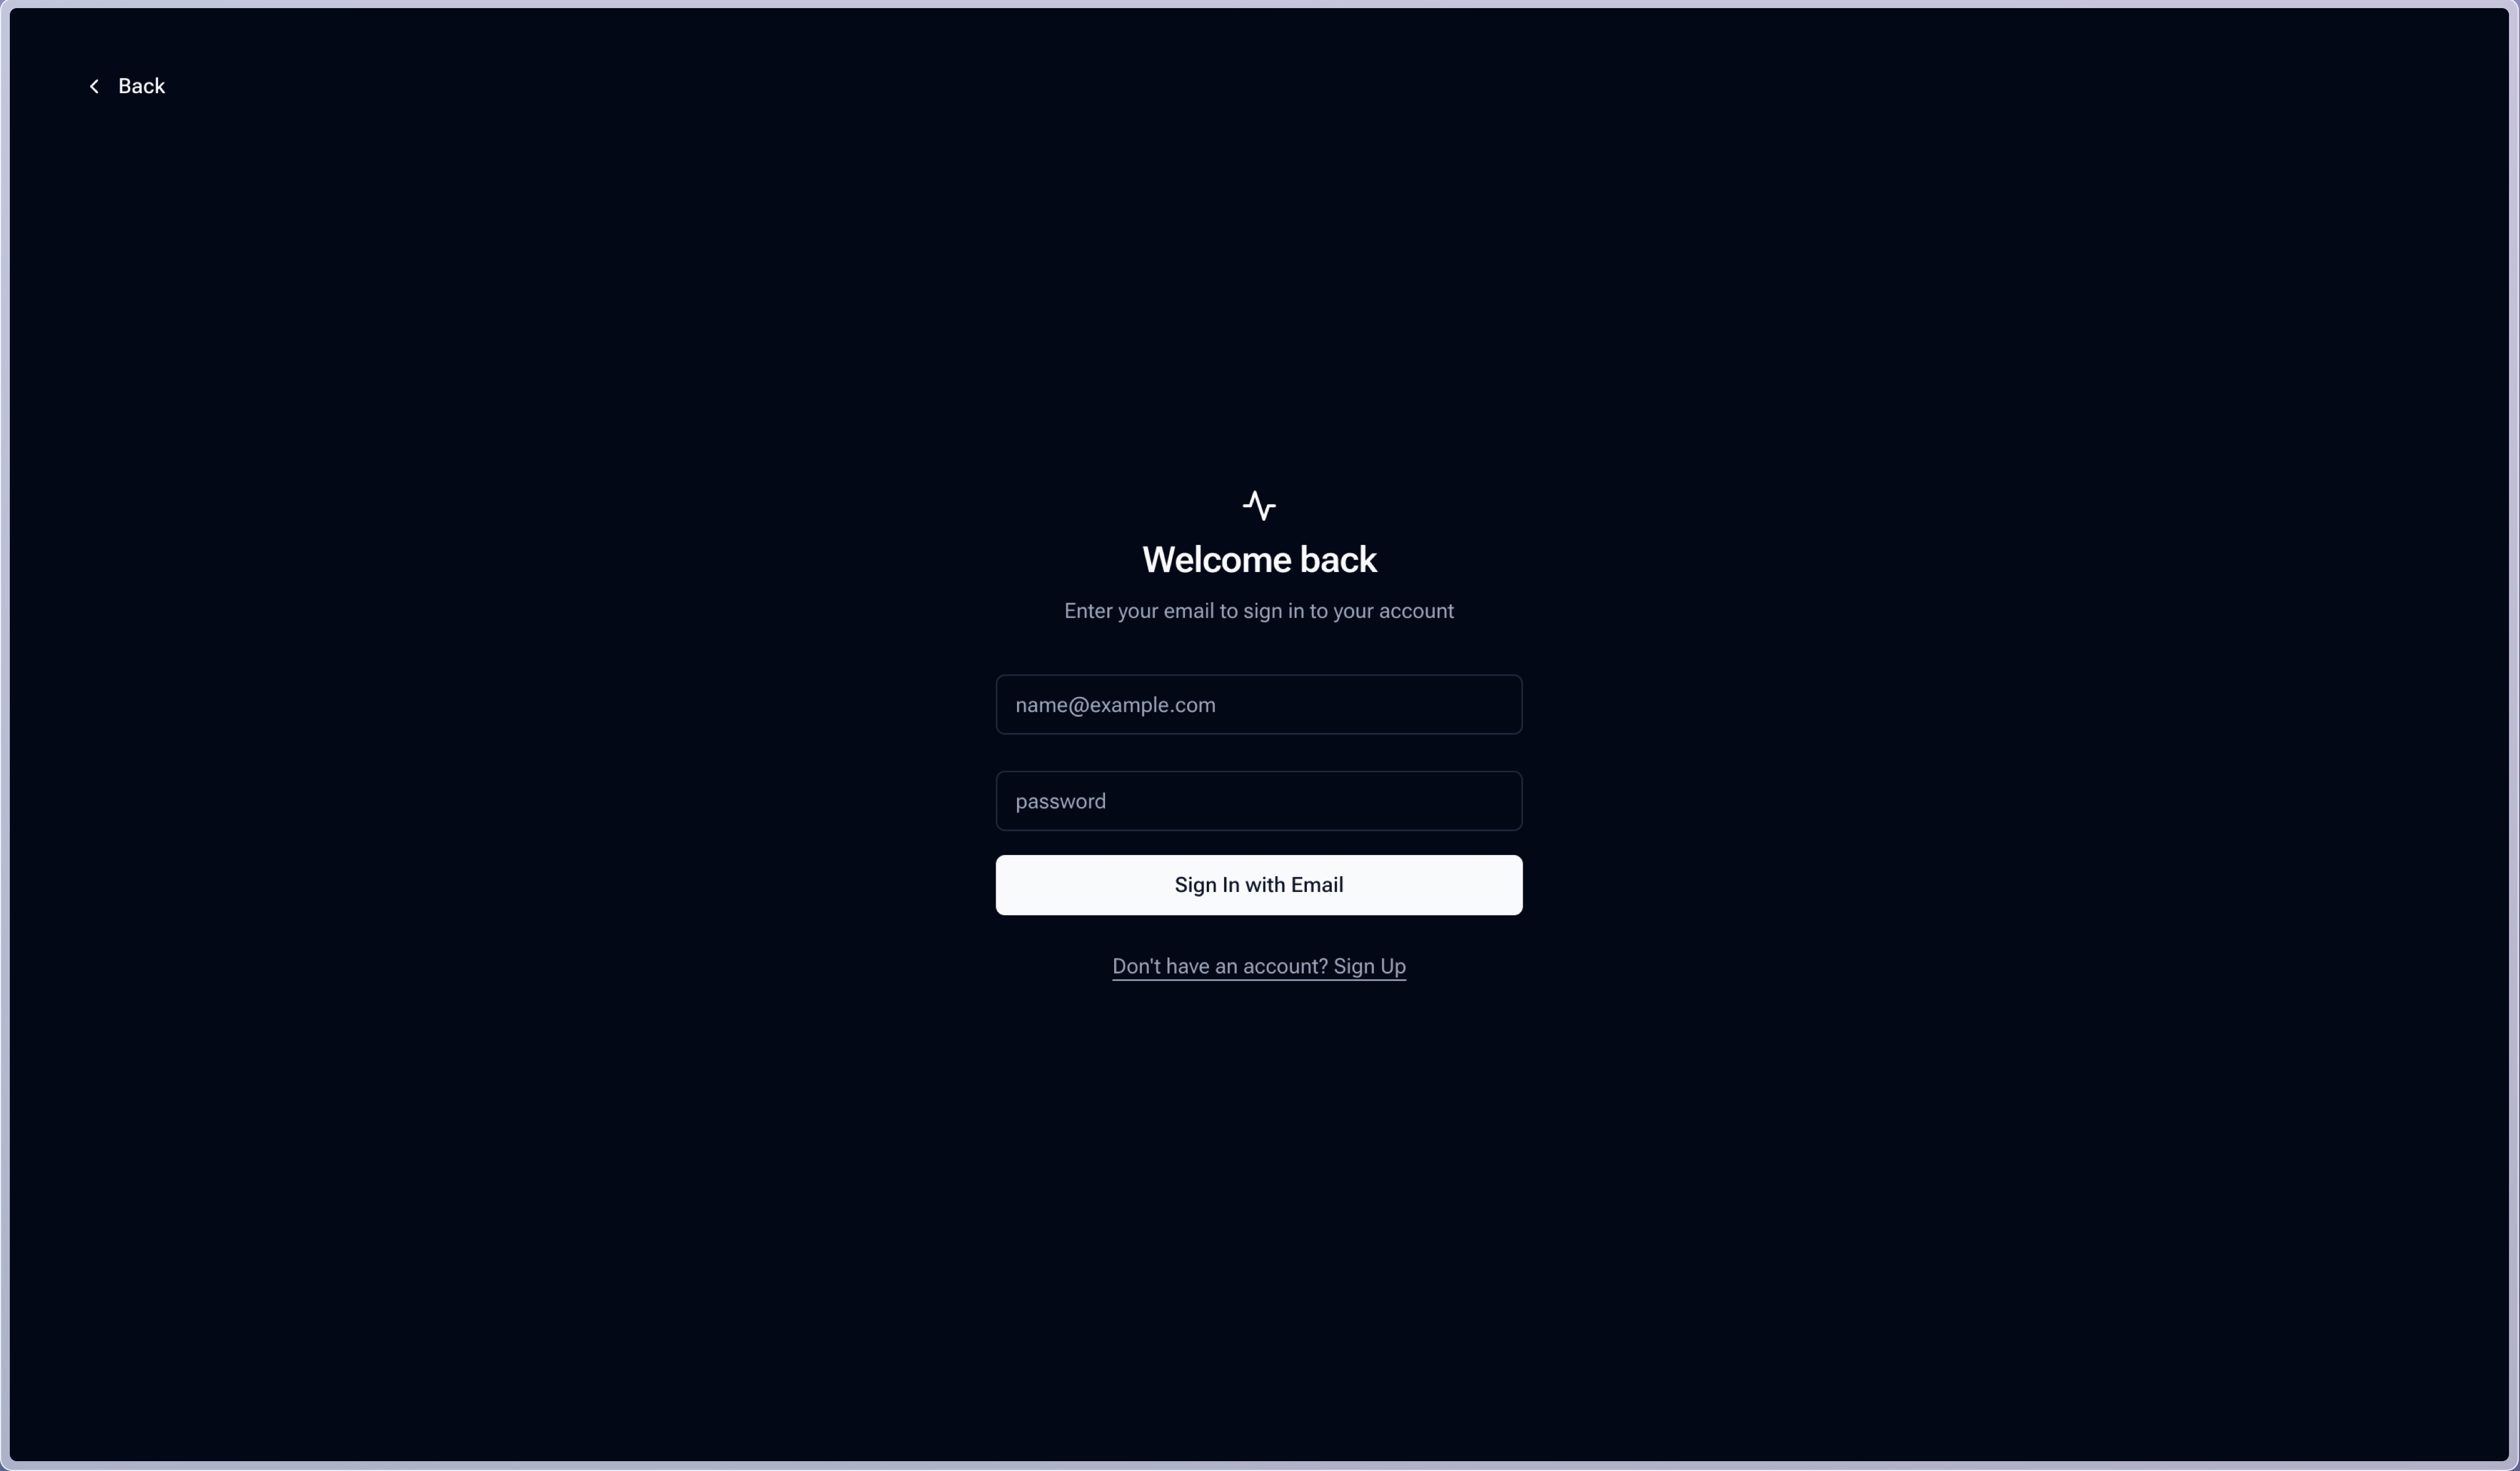
\includegraphics[height=6cm]{figures/fyp_login.jpeg}
  \captionsetup{justification=centering}
  \caption[Web app Login]{The login screen for the web app} \label{fig:webapp_login}
\end{figure}
When users first navigate to the website, they are greeted with either the login screen (\autoref{fig:webapp_login}), or the register screen (\autoref{fig:webapp_register}). The login screen is simple, with only two fields, one for the user's email address, and one for their password. The register screen is similarly simple, with fields for the user's name, email address, and password. Users are also required to agree to the consent form and acknowledge they have read the information sheet provided by a PDF link. The consent form and information sheet were written as part of the ethics approval obtained to collect user information. Once the user has registered, they are automatically logged in and redirected to the dashboard screen.
\begin{figure}[htbp]
  \centering
  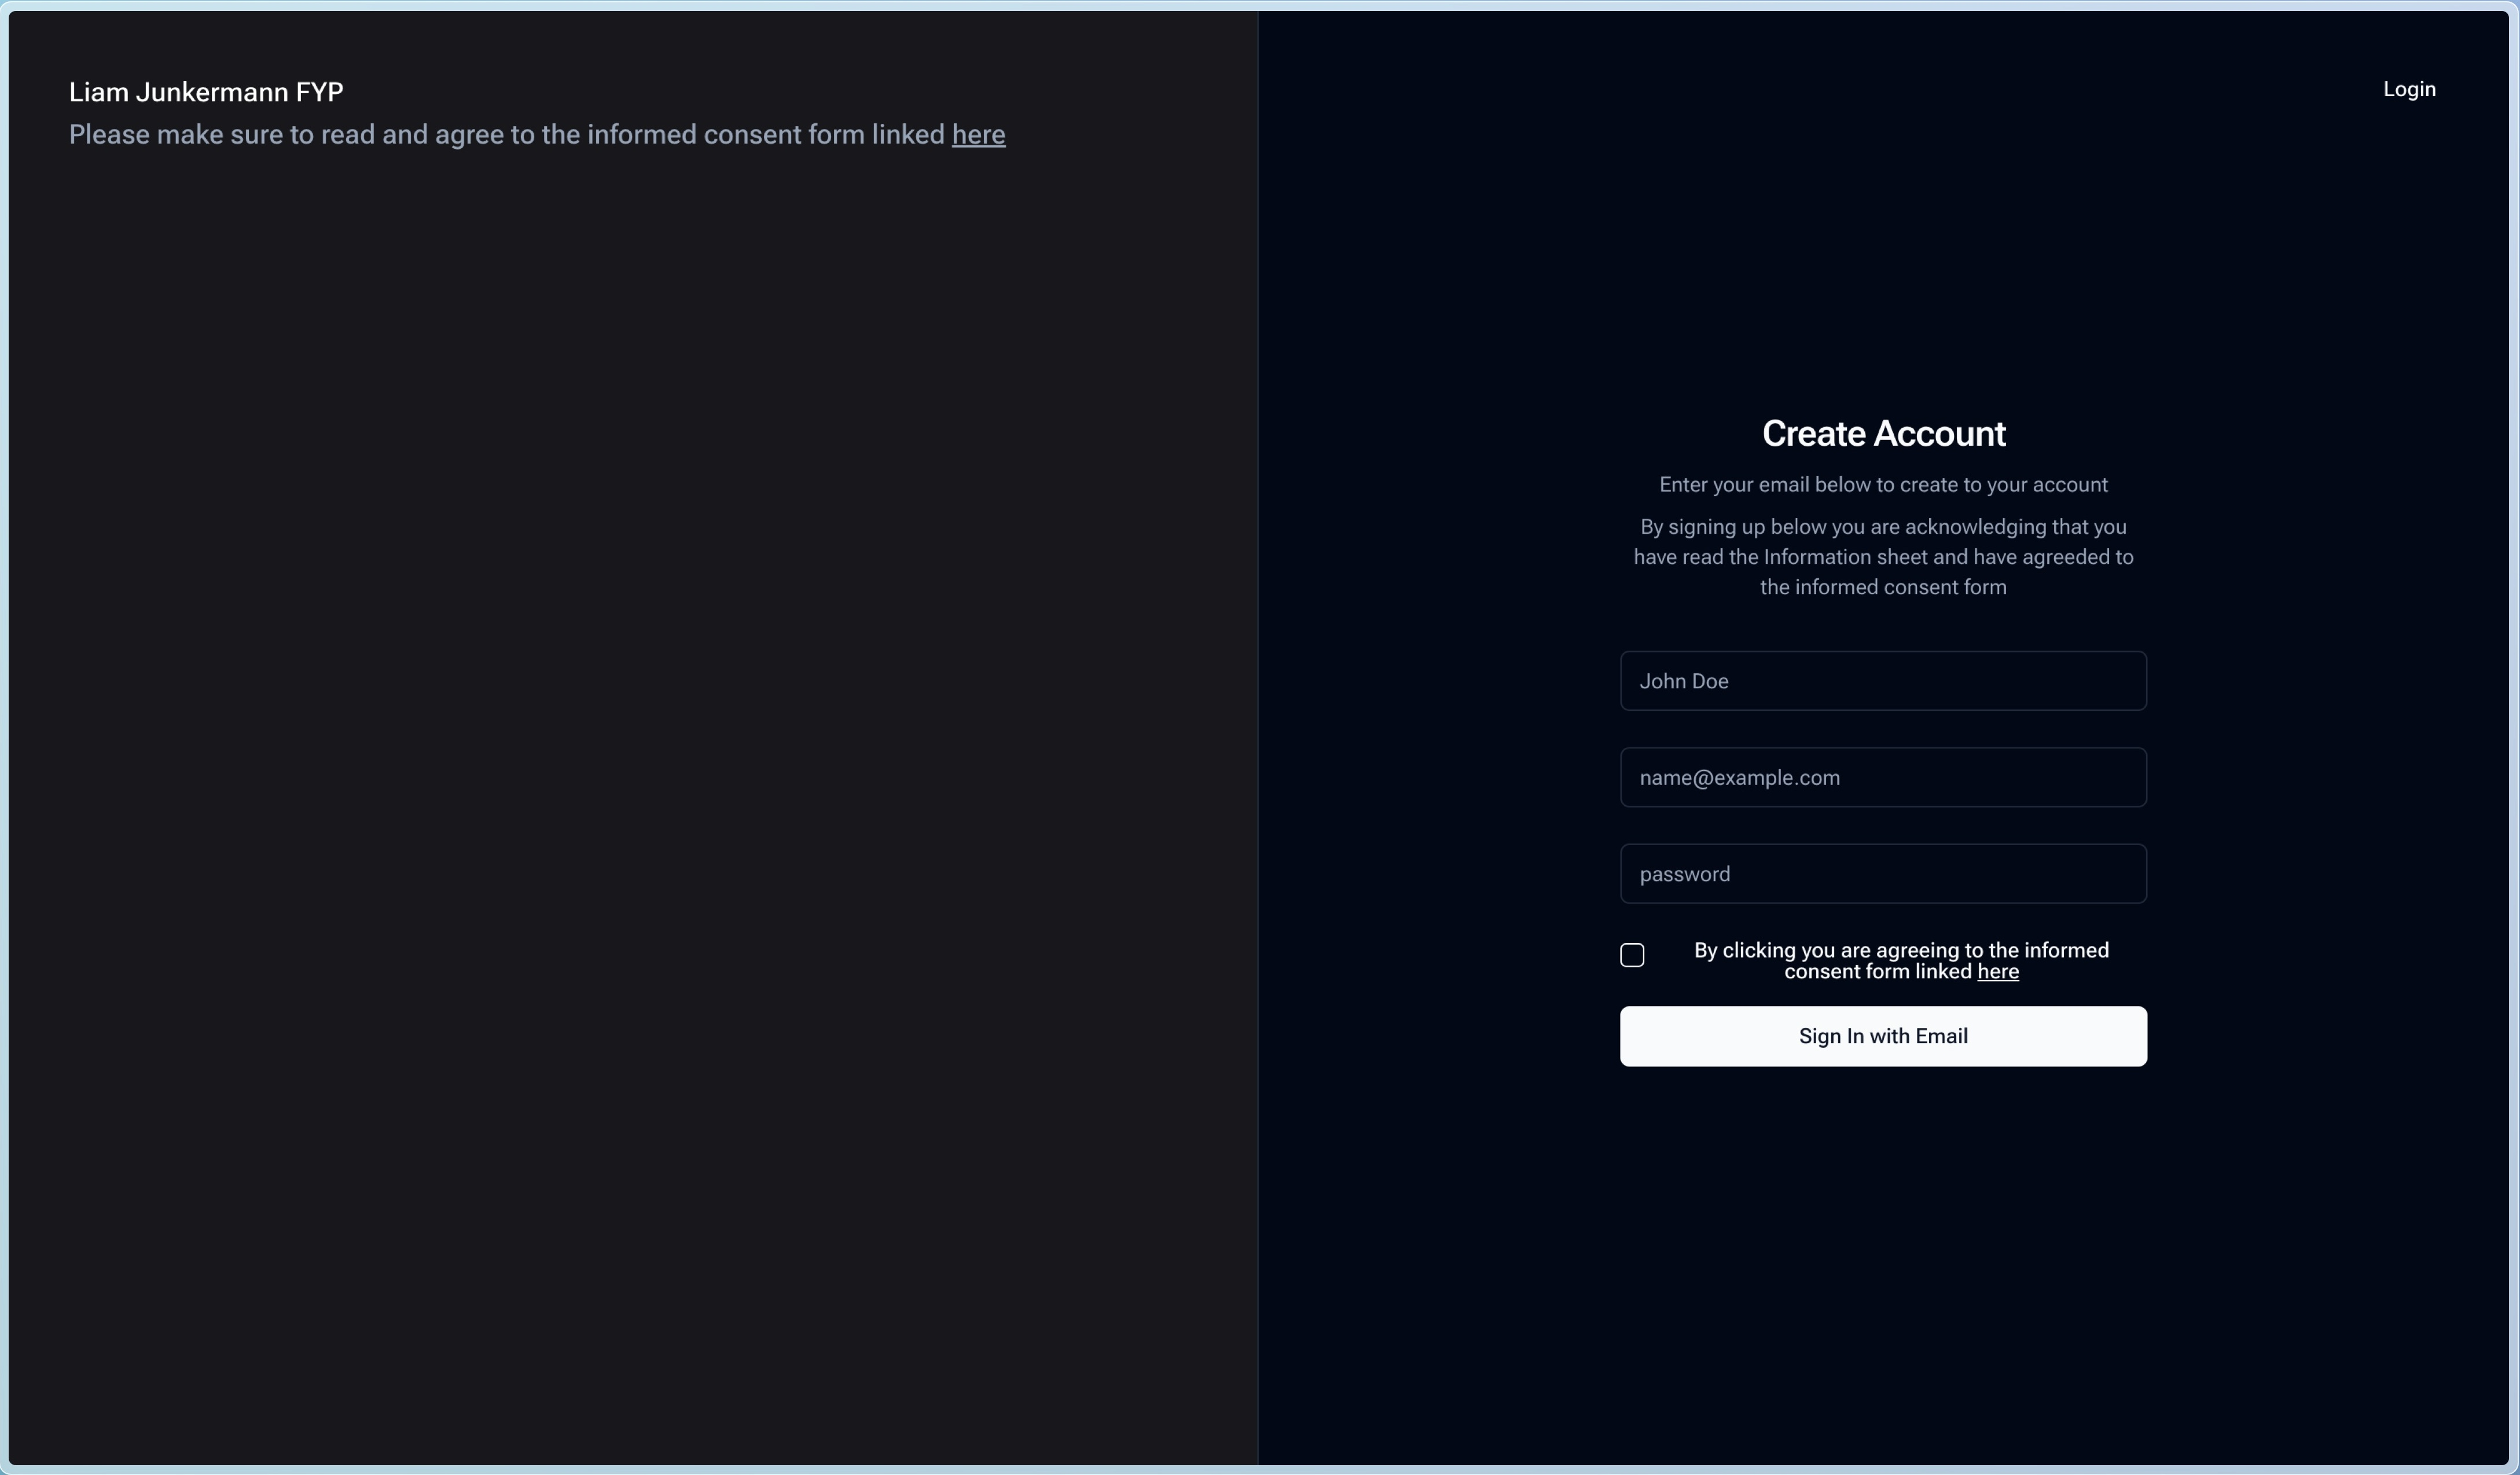
\includegraphics[height=6cm]{figures/fyp_register.jpeg}
  \captionsetup{justification=centering}
  \caption[Web app Register]{The user registration screen for the web app} \label{fig:webapp_register}
\end{figure}
\subsubsection{Dashboard}

\begin{figure}[htbp]
  \centering
  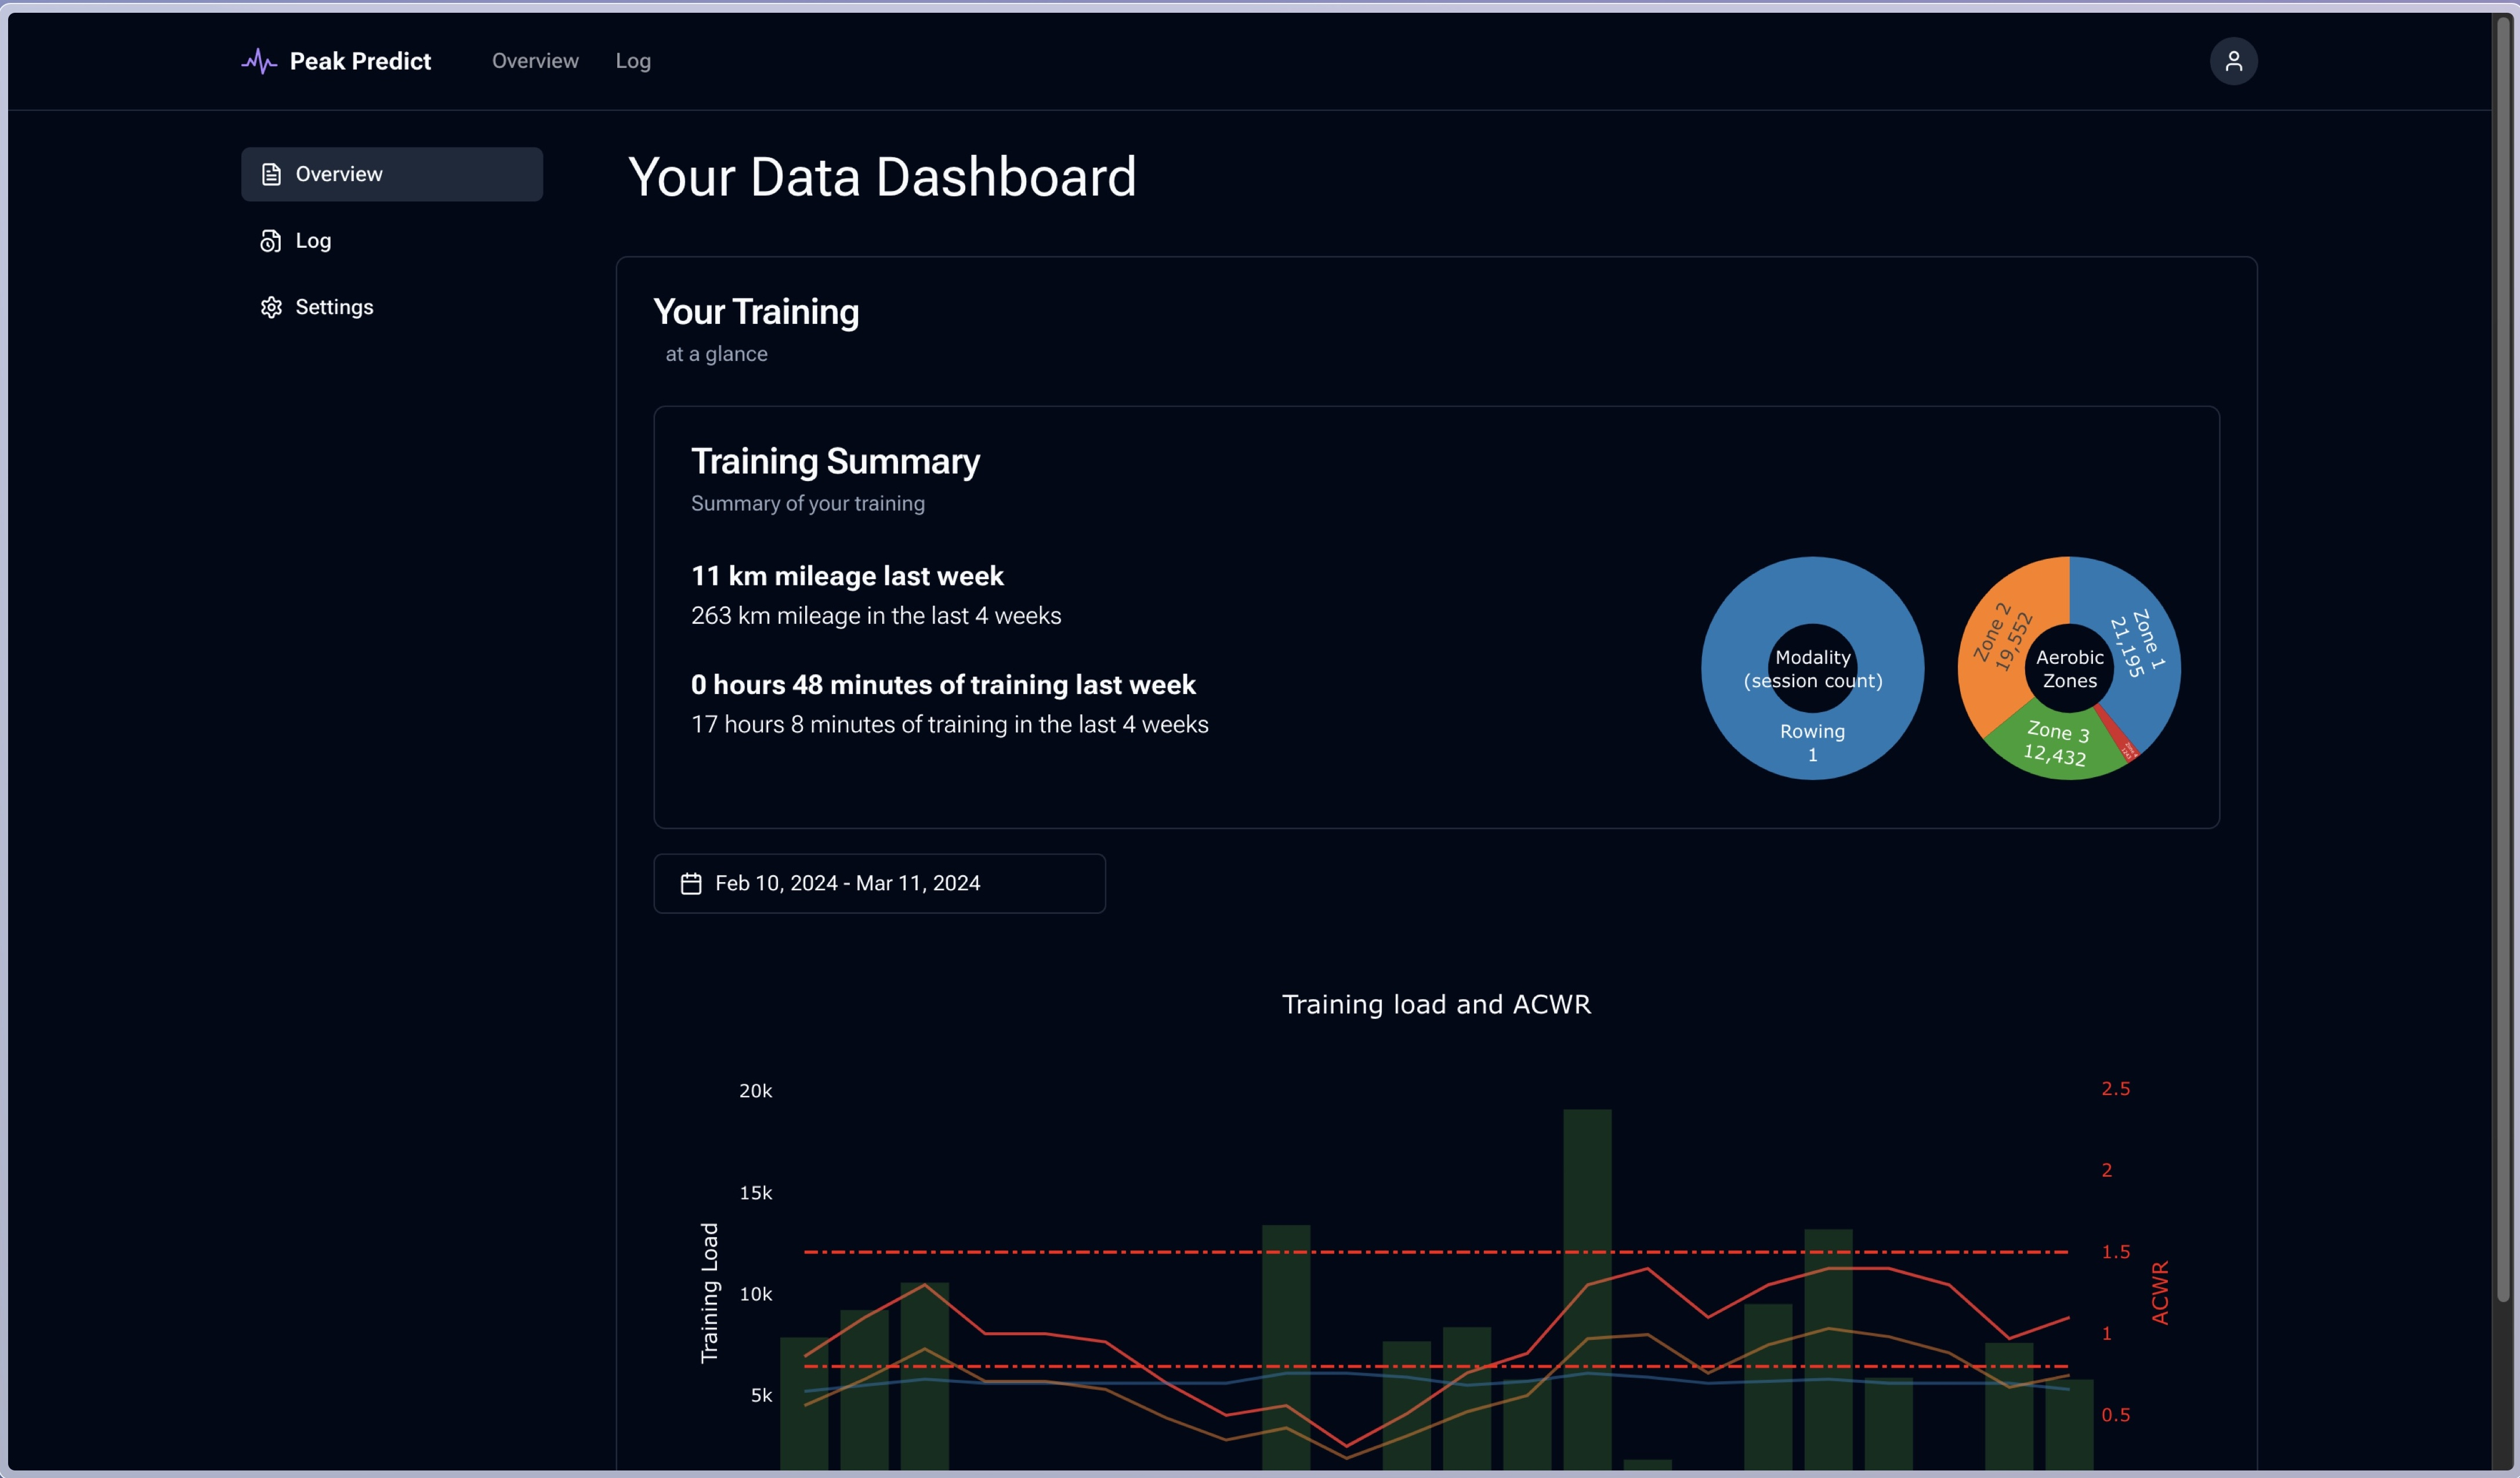
\includegraphics[height=6cm]{figures/fyp_dash_overview.jpeg}
  \captionsetup{justification=centering}
  \caption[Web app Dashboard]{The dashboard screen for the web app} \label{fig:webapp_dashboard}
\end{figure}

Once logged in, users are greeted with a dashboard screen (\autoref{fig:webapp_dashboard}). This screen gives a summary of training in the last seven days, as well as some visualisations across a selected time period of the user's choice. At a glance, athletes are able to identify if they are training sustainably, and compare, week-to-week, their mileage and modality break-down. Managing training load is particularly important for rowers as overtraining has even greater knock-on effects in other aspects of a rower's life, like work or college. 

\subsubsection{Training log}

\begin{figure}[htbp]
  \centering
  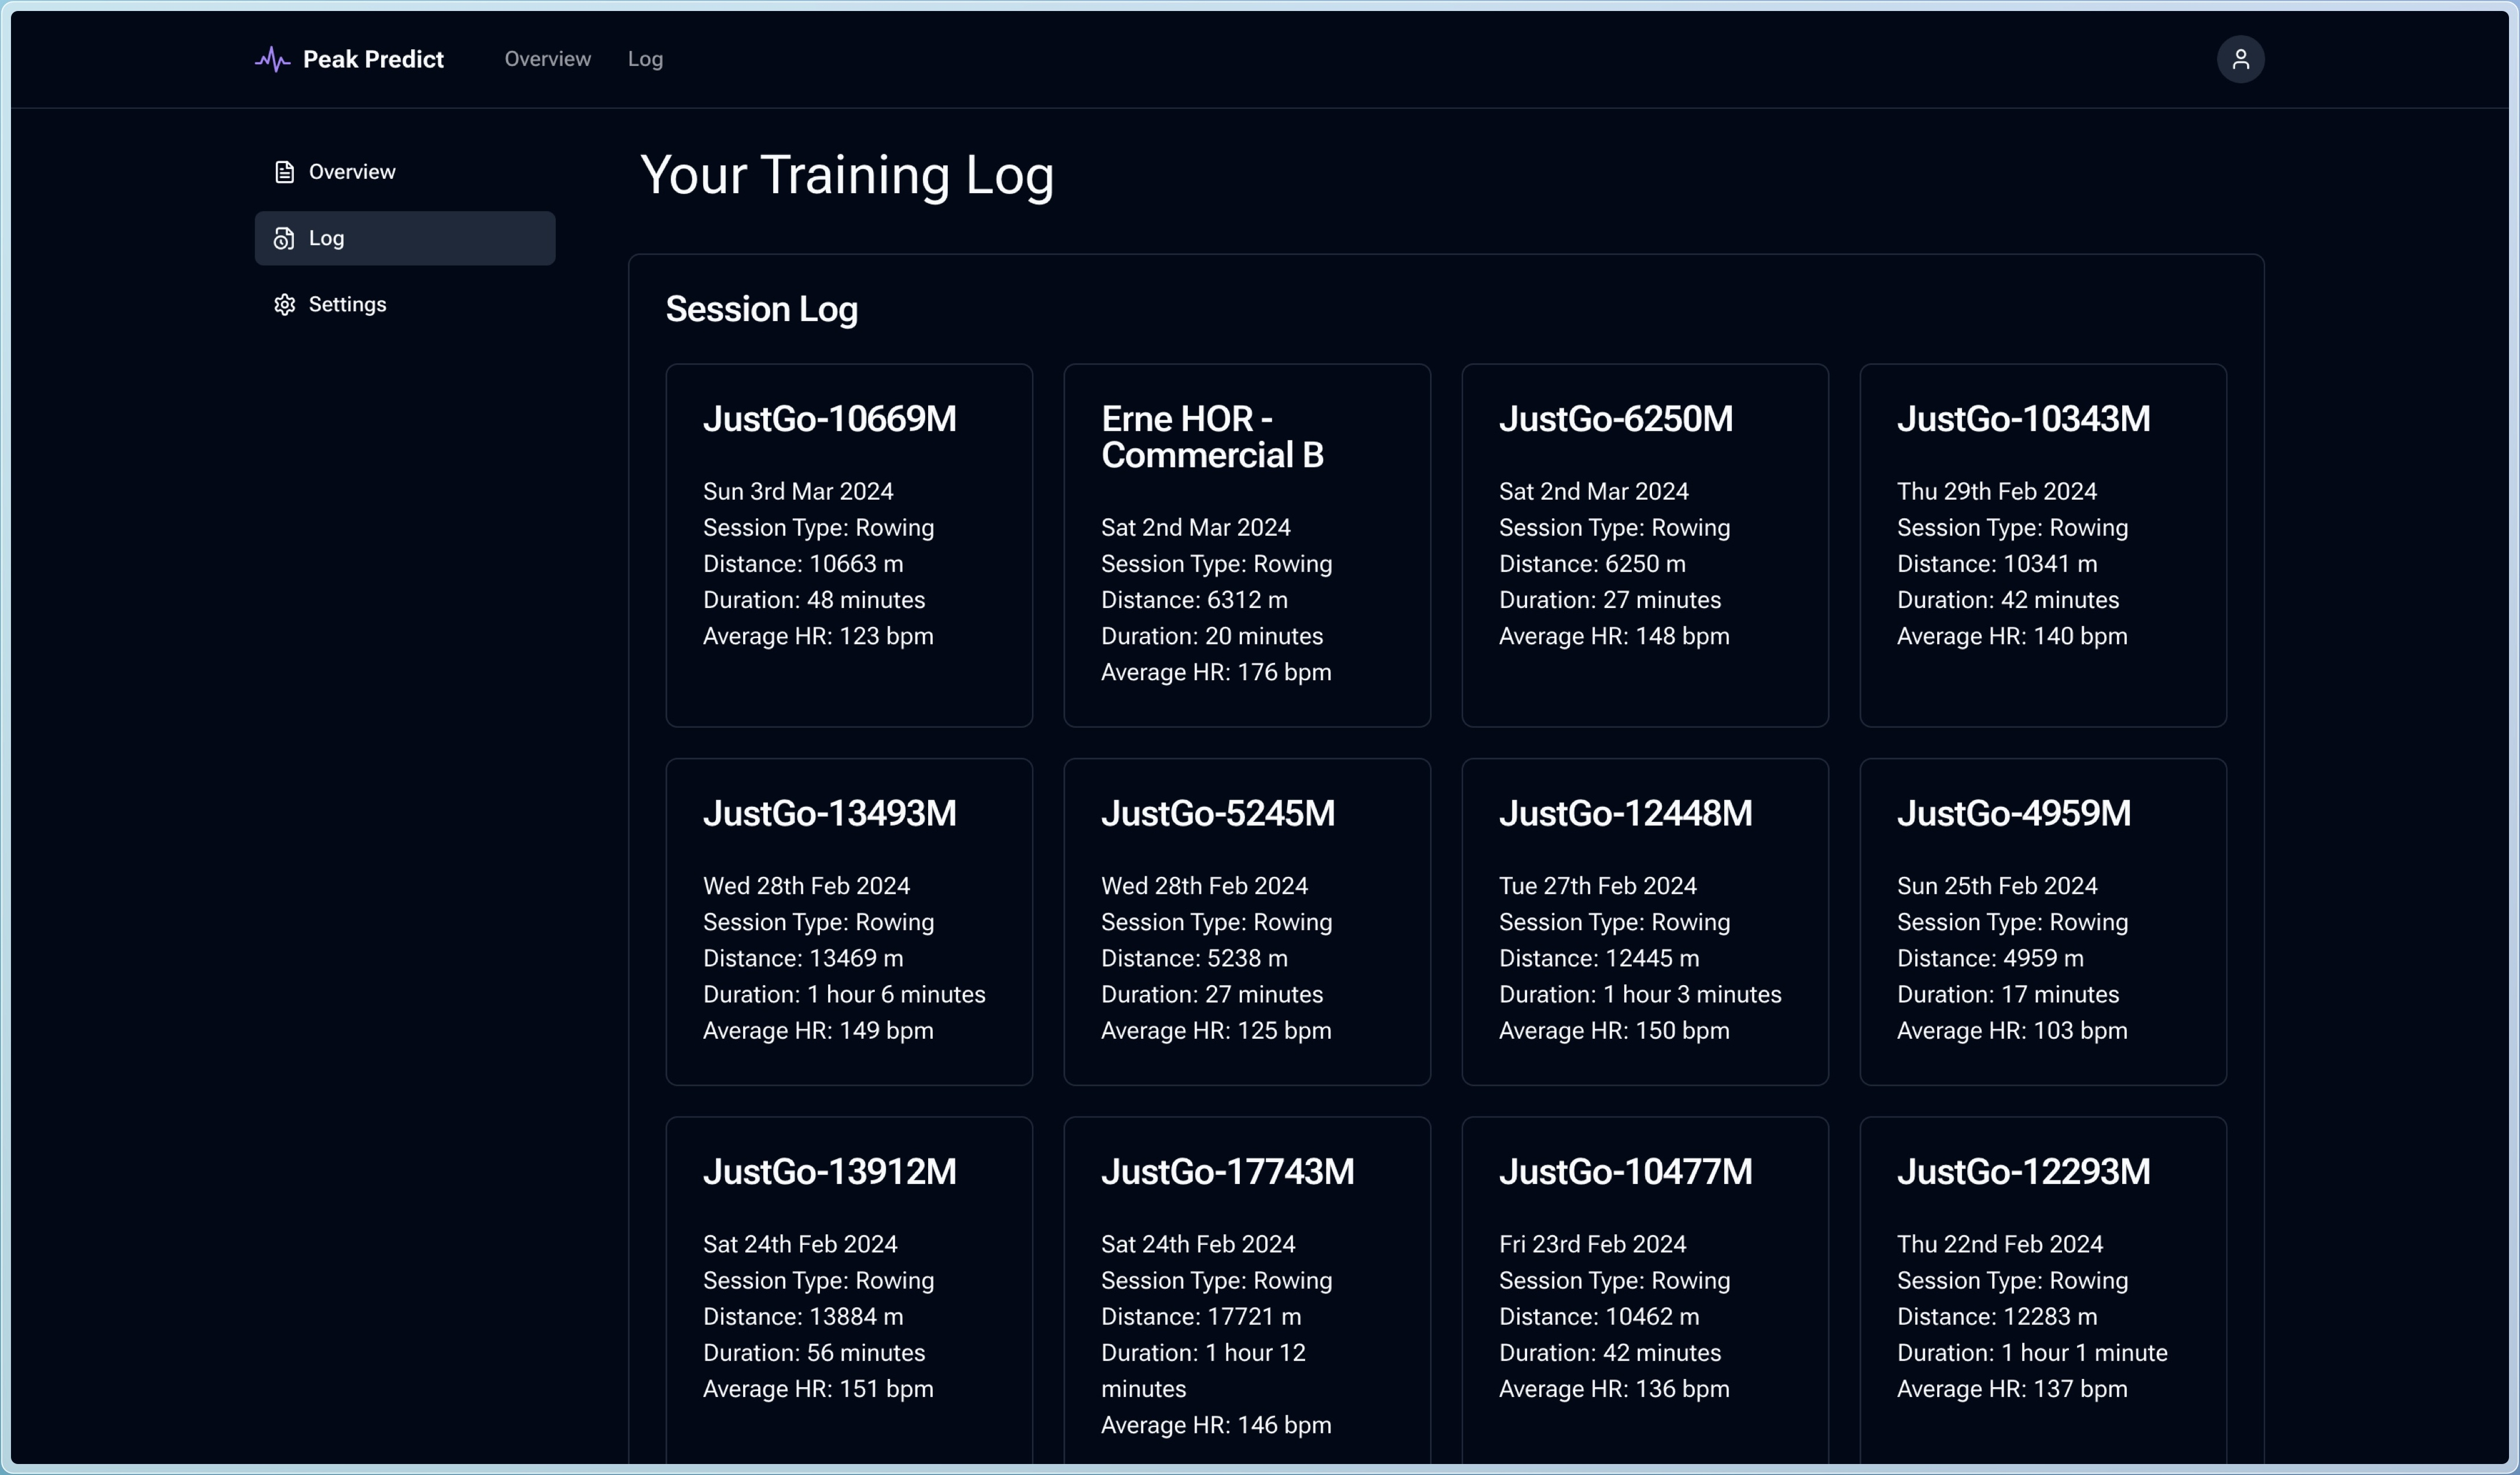
\includegraphics[height=6cm]{figures/fyp_training_log.jpeg}
  \captionsetup{justification=centering}
  \caption[Web app Training Log]{The training log screen for the web app} \label{fig:webapp_training_log}
\end{figure}
The training log (\autoref{fig:webapp_training_log}) provides a detailed view of all the sessions a rower has completed. This project did not require athletes to provide additional feedback for sessions, however, this page would host a form to allow athletes to add sessions and session feedback in a more developed version of the web app, this will be discussed more in the Discussion, \autoref{chap:discussion}. The user can also click on a session to view more detailed information about that session, including heart rate data, GPS data, and any other data collected during the session. 

\subsubsection{Connections manager}

\begin{figure}[htbp]
  \centering
  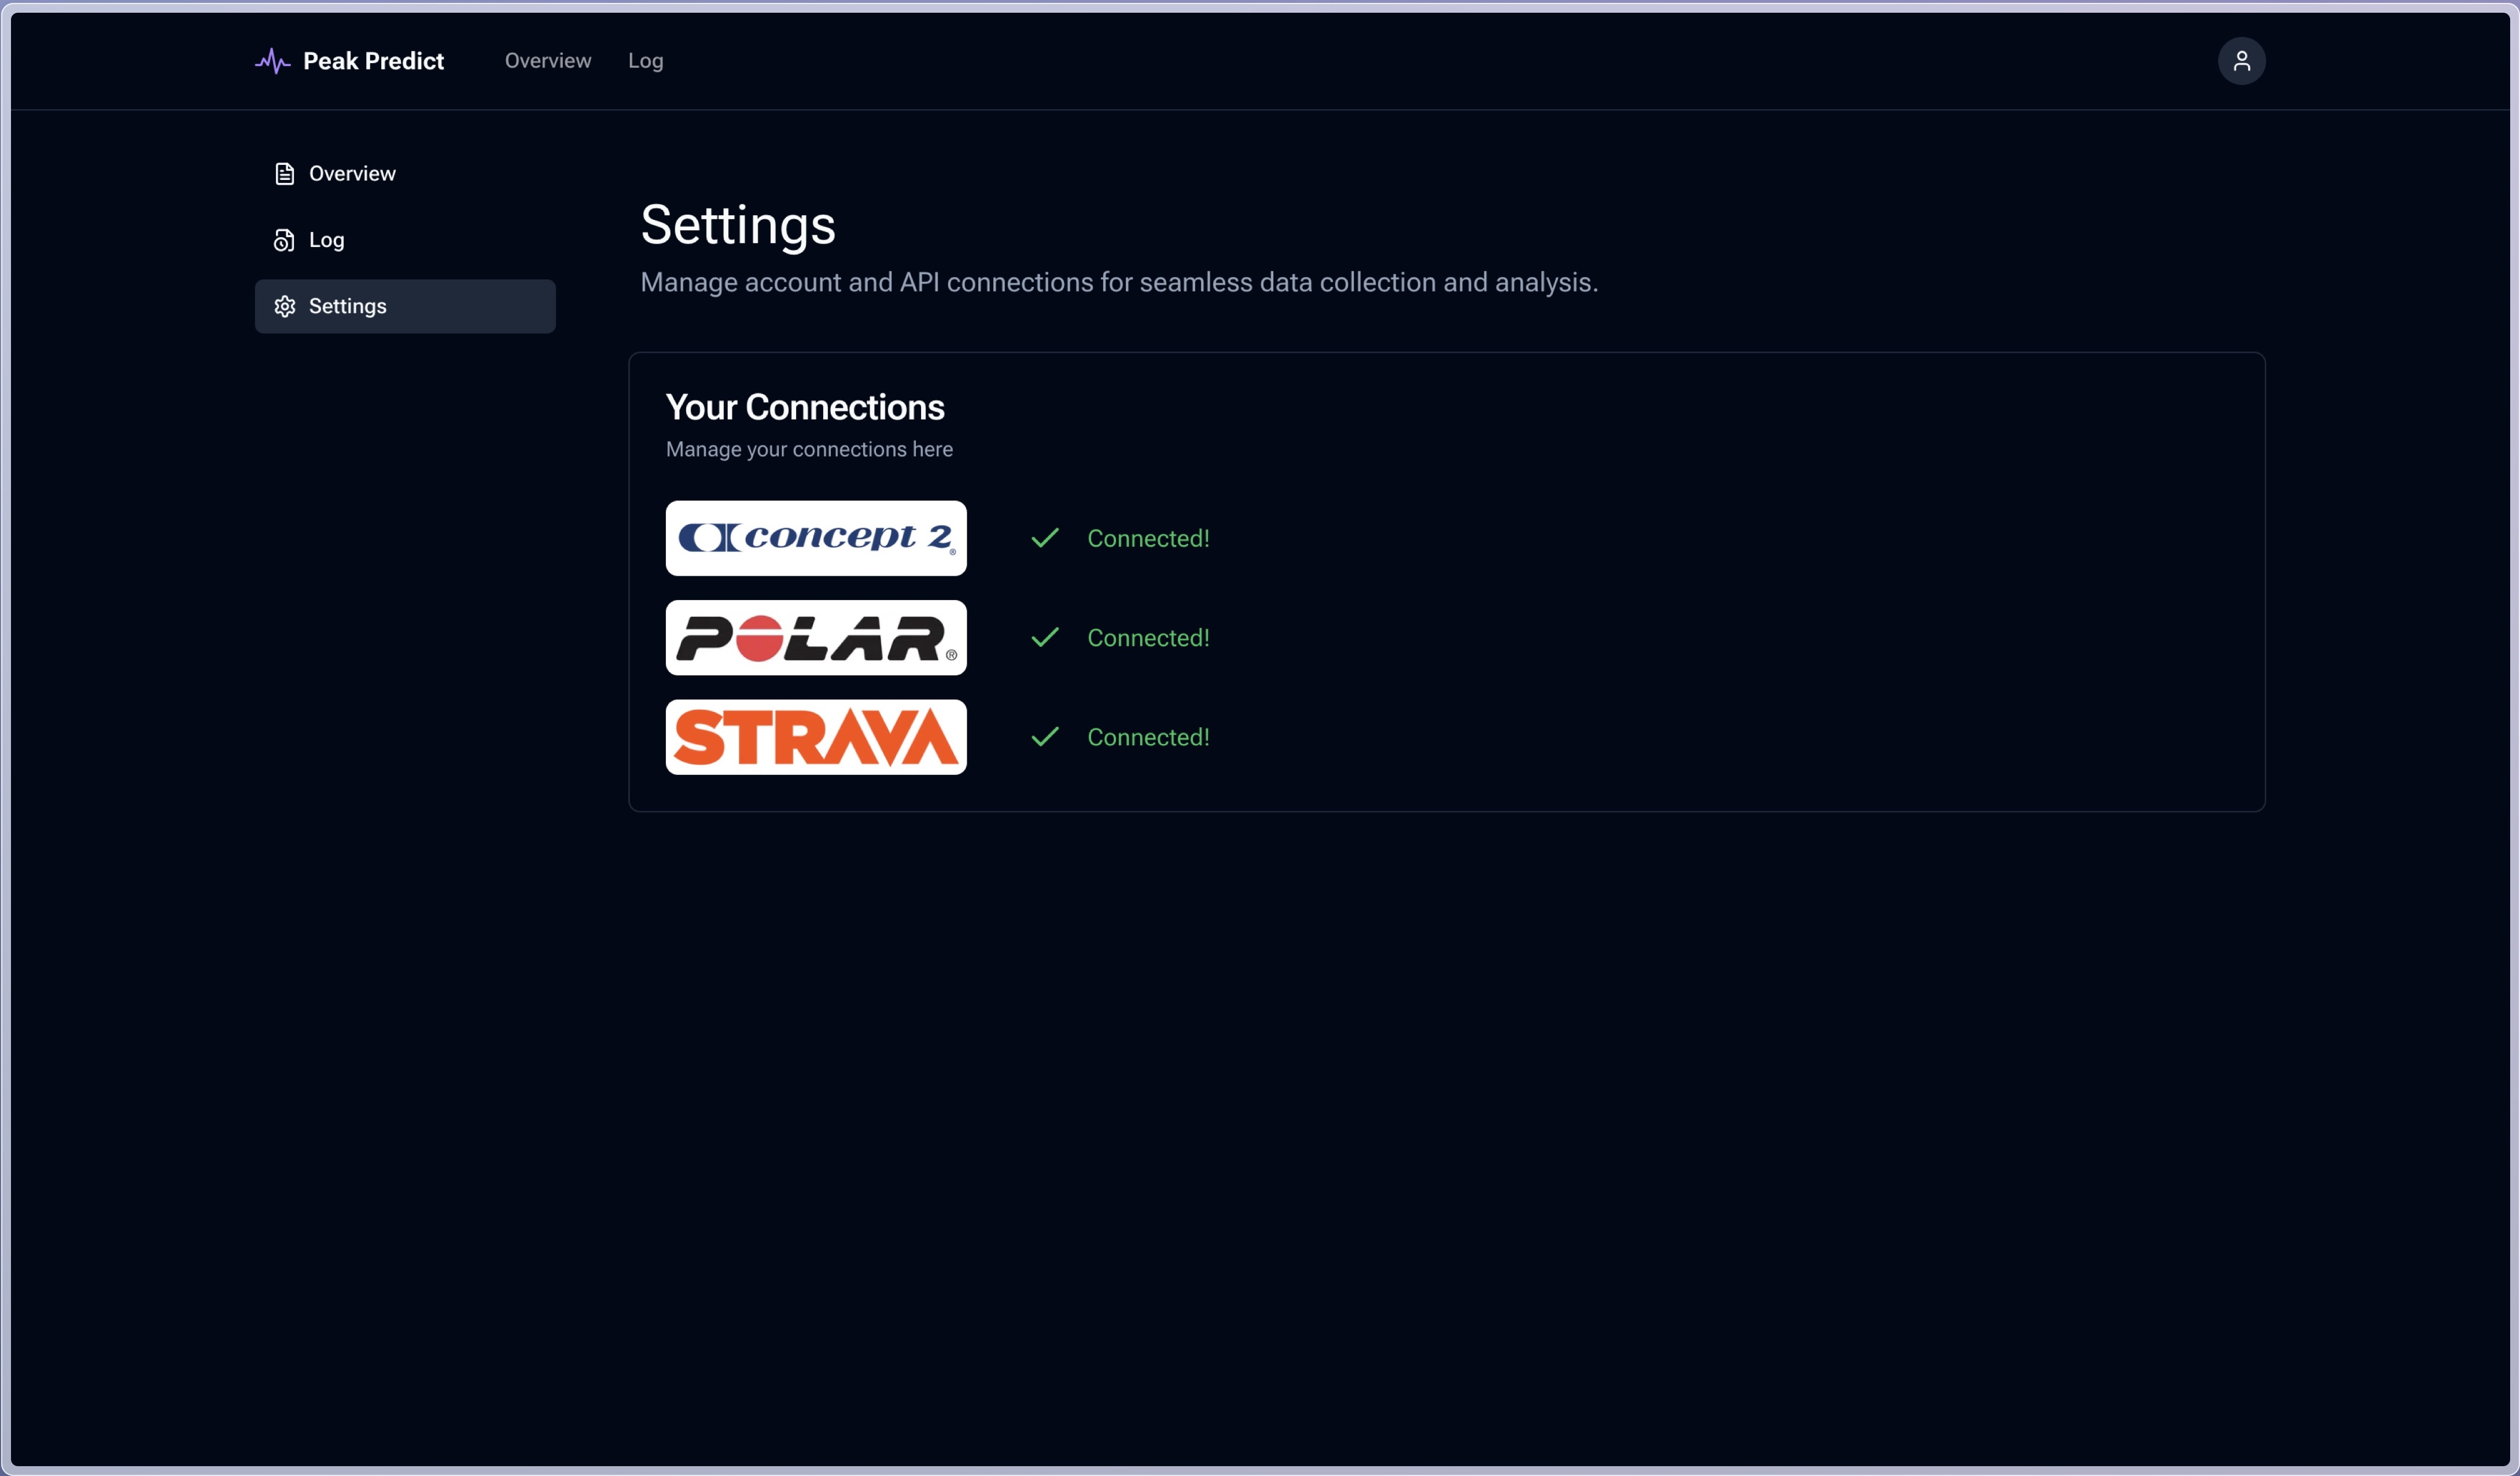
\includegraphics[height=6cm]{figures/fyp_connections_page.jpeg}
  \captionsetup{justification=centering}
  \caption[Web app Connections Manager]{\label{fig:webapp_connection_mgr}The connections manager screen for the web app} 
\end{figure}
The final screen in the app is the settings page (\autoref{fig:webapp_connection_mgr}), which is home to the connections manager. Here users can see which data providers they have connected. This page is where the most user interaction happened throughout the project. Given the goal of minimal user intervention and maintenance, when logging in for the first time they were directed to this page to connect their rowing data providers, and using the OAuth protocol, shared the necessary keys with the project to allow data to flow automatically in the backend.  

\subsection{The Backend}
The backend services were crucial to developing a system that required minimal user and maintainer intervention. The backend was developed using serverless functions, which are small, single-purpose functions that are run in response to events. These functions were used to collect data from the user's data providers, analyse the data, and generate feedback for the user. The backend was developed using the Serverless framework, which is a framework for building serverless applications. The backend was hosted on AWS and used a combination of AWS Lambda, AWS API Gateway, AWS DynamoDB, and AWS S3 to provide the serverless functions and store the data. The backend functions were primarily built using Node.js and Typescript. This section will only discuss the data collection and management functions. Analysis functions will be discussed in the Data Analysis and Visualisation chapter, \autoref{chap:data-analysis-viz}.

There are 4 major functions, which were separated into serverless functions to manage and handle data. These functions are the Provider Connection, Provider Webhooks, Data Ingestor, and Data Processor. Each of these functions is responsible for a different part of the data collection and management process.

The general web app backend was mostly handled by AWS Amplify. This service made it possible for the researcher to focus on providing valuable features to users, rather than spending extra time developing boilerplate authentication and database interactions. The Amplify service also provided a GraphQL API, which was used to interact with the DynamoDB database, and provided a simple way to interact with the database from the frontend in a secure way.

\subsubsection{Provider connection}
When connecting to a service using the OAuth protocol, the user is redirected to the service's login page, where they log in and authorise the project to access their data. Once the user has authorised the project, the service redirects the user back to the project's website and provides an access token that can be used to access the user's data. This access token is then stored in the database and is used to access the user's data in the future. This function is responsible for handling the OAuth flow and storing the access token in the database. The provider connection function handles the various data formats which different providers use, and connects access and refresh tokens to the users for use later on in the pipeline when activities are generated. This particular function was built as part of the Next.js server, leveraging the server-side rendering capabilities of the framework to handle authentication of users using cookies making the linking of tokens with users easier.

\subsubsection{Provider webhooks}
Typically when a user completes a workout, the data provider can query a webhook (if it has been set up), with a payload containing basic information about the workout, and in some cases, the details to retrieve the full session. For each of the supported data providers, Polar, Concept2, and Strava, webhooks were setup and registered with the providers. Webhooks were then handled through the Next.js server, retrieving any additional data needed. The full session data was then shared to the Data Ingestor function for processing and storage in the database. Different providers had different requirements for the webhook payload, and the data was stored in different formats, so the webhook function was responsible for handling these differences and normalising the data before sending it to the Data Ingestor function, while also limiting the unnecessary sharing of client secrets and keys across multiple services.

\subsubsection{Data ingestor}
The data ingestor handled the actual storage of the data in the database. The data ingestor first validated any data provided. This was done by validating the provider user id and comparing a key which was shared with the Next.js server. Then it stored the raw session data, provided by the webhook handler in the Next.js server, in AWS S3, this meant that any issues with data processing could be rectified after the fact with the raw data available. Finally, the ingestor triggered the Data Processor function. This extra level of data processing before storing the data ensured that data ingested to the data pipeline was legitimate and provided through the proper channel. This function was a standalone serverless function, built using Node.js and Typescript, and deployed to AWS Lambda using the Serverless framework.

\subsubsection{Data processor}
Given the variety of data and session types provided, a standard exercise model was needed to make analysis and machine learning easier. This standard exercise model will be discussed in more detail in the data cleaning section of the data analysis chapter (\ref{sec:data-cleaning}), with a schema introduced in the Data management section of this chapter (\ref{sec:data-mgmt}). The data processor function was responsible for taking the raw session data, and converting it into a standard format. The standard format included a sessions duration, distance, average heart rate (if applicable), time of completion, session type, and session modality. These features would be used to complete analysis and produce the weekly training summaries shown in the front end. This was also a standalone serverless function, built using Node.js and Typescript, and deployed to AWS Lambda using the Serverless framework.

\section{\label{sec:data-mgmt}Data Management}
Given the expected volume of data collected, the design of how to store and manage this data was important to ensuring analysis could happen quickly, and AWS costs remained low. Almost all the data stored was already provided in a structured JSON format, originally these data responses were saved and stored in AWS S3. This allowed the researcher time to understand what data was being collected, and what was important. From this, the Standard Exercise Model was derived. The process for how this model was developed will be detailed in the next chapter \ref{chap:data-analysis-viz}. This model was then used to create a DynamoDB table to store the data in a structured format. The data was stored in a table with the schema described in \autoref{tab:std_exercise_model}.
\begin{table}[h]
  \centering
  \resizebox{\textwidth}{!}{%
  \begin{tabular}{lll}
  \textbf{Column Name} & \textbf{Column Data Type} & \textbf{Description} \\
  \texttt{owner} & \texttt{string} & The users uid \\
  \texttt{exercise\_id} & \texttt{string} & An autogenerated id. The tables primary key \\
  \texttt{data\_source} & \texttt{\{source:~string, path:~string\}{[}{]}} & The raw data source(s) and linked data in S3 \\
  \texttt{datetime} & \texttt{number} & The unix timestamp for the session \\
  \texttt{type} & \texttt{"endurance" | "interval" | "strength" | "other" | "unknown"} & The session type, an enumerated list \\
  \texttt{modality} & \texttt{"row" | "erg" | "other"} & The session modality, an enumerated list \\
  \texttt{duration} & \texttt{number} & The duration, in seconds, of the session \\
  \texttt{distance} & \texttt{number} & The distance, in meters, of the session \\
  \texttt{avg\_hr} & \texttt{number} & The average HR, in bpm, of the session
  \end{tabular}%
  }
  \caption[Standard Exercise Model Schema]{\label{tab:std_exercise_model}The schema for the "Standard Exercise Model"}
\end{table}

This schema made it particularly easy to perform analysis on each athlete's training, distilling the key metrics into a small data size. DynamoDB also allows for robust querying of large datasets, allowing this solution to scale well with lots of data. The data was stored in a single table, with the \texttt{exercise\_id} as the partition key, and the user's unique id (\texttt{owner}) as the sort key. This allowed for easy querying of the data and made it easy to retrieve data for a specific user, or for a specific session. With connections to the raw data included in this data format, more detailed analysis can still be completed automatically, without unnecessary S3 reads to find the session amongst a larger, less dynamic data set. Future work could continue to grow this standard model, adding more features which may be commonly used for analysis, such as time in zones, calculated training impulse, or more. However, for the purposes of providing data for the frontend and the initial analysis, this model was sufficient.


\chapter{Data Analysis and Visualization} \label{chap:data-analysis-viz}
Collecting and managing data is a key part of this project, although simply collecting data does not provide any benefit to athletes. Data analysis and visualization are essential to extract useful information from the data. This chapter will discuss the data analysis and visualization process, including cleaning of the data collected, the analysis performed, and the visualizations generated and presented as feedback to users.

\section{Data Cleaning}\label{sec:data-cleaning}
The data collection step was developed to reduce any cognitive load for users. As a result, there are a number of data sources, and therefore a number of data formats, which need to be cleaned and transformed into a uniform format for further analysis. Furthermore, some athletes might use a number of devices to track a session, so it is also necessary to match multiple session results to a given session. All the raw data from the data providers was stored throughout the project in case the data cleaning steps changed; this allowed database tables to be as small, and queryable, as possible.
\subsection{Identifying valuable data}
In order to begin data cleaning, it was important to understand what information was valuable. In order to do this, collected data was analysed for what information was available across each session provided, then understanding what basic analysis and feedback would be most useful to athletes. The most basic information clearly needed is the date and time of a session, what modality of session it is (row, ergometer, or other), and what type of session it is (endurance, interval, strength). These modalities and types were intentionally kept quite simple, with only three options, in order to make analysis easier to start. Next, in order to do any kind of fatigue or training impulse analysis, the duration of a session needed to be considered, along with any available heart rate or RPE information. Finally, rowers measure progress in training through mileage so a session's mileage, where appropriate, was included in this standardised model. As a result of this brief macro-analysis of the data and expected analysis results, the "Standard Exercise Model" described in the previous chapter (\autoref{tab:std_exercise_model}) was generated.

\subsection{Developing a cleaning process}
The data collection pipeline ingests sessions regardless of type. This required a series of functions to handle data from different providers and perform analysis on session data to appropriately classify each session, and normalise to the standard exercise model developed in the previous chapter.

\subsubsection{Identifying session modality}
The first step in cleaning data was identifying the session's modality. Was a session a row, an erg, or something else? Typically the sessions were tagged, with sessions coming from Strava being classed as "rowing", regardless of if they were on the water or on the rowing machine, causing some issues. Sessions not explicitly tagged by Strava, for example, or ingested from Concept2 were initially flagged as other. This approach, however, did result in some issues. One member of the Commercial Senior Squad, for example, uses a running watch which classifies on-the-water sessions as runs. He also happens to be an avid runner so it was necessary to analyse sessions to determine if they occurred on land or on water. As a result of this case, and the issues with differentiating on the water or on the machine "rowing" from Strava, it became clear a more developed approach was necessary to accurately identify session types. Differentiating on-the-water rows and erg sessions was much easier. In many cases, erg sessions were provided through the Concept2 API and were easily identified. On-the-water rows were typically provided through Strava and were identified by the activity type and generally the presence of GPS data. Users who did not have a GPS in the boat could manually insert sessions and the name of the session could be used to identify the modality.


\subsubsection{Identifying session type}
The next challenge in the data cleaning process was determining if a session was an endurance or interval session. Typically, the distance and duration can be used to identify a session. For erg sessions provided through the Concept2 API, distance, time, watts, and pace were included at a minimum. It is possible to differentiate endurance or interval sessions when comparing pace with other sessions from that user. The ideal session data from Concept2, though, includes highly detailed information about a session such as distance, duration, average wattage, pace, and heart rate, and detailed stroke-by-stroke data including wattage, pace, and heart rate. Many athletes, though, choose not to connect a heart rate monitor to their rowing machine, so it was necessary to match heart rate data, recorded through Polar, with the stroke data, when available. Using heart rate it is very easy to identify if an erg session is an interval or endurance session.

Identifying the type of an on the water row was more difficult. Some on-the-water sessions may be a mix of interval and endurance. A common training session for the researcher throughout this project was 10 kilometres of endurance paddling, followed by 10 kilometres of interval work. In this case, the session could be classified as an interval session. The researcher, however, would separate this into two sessions, classifying the first 10 kilometres as endurance training, considering the duration and average heart rate, and the second 10 kilometres as interval training, again considering the duration and average heart rate to calculate the training impulse. This is a clear example of the limitations of the data collected. The researcher could manually classify this session as an endurance session, but this would not be scalable. A model could be developed to classify this session, but unfortunately, not enough data was collected and classified to warrant the time needed to develop the model. As a result, the approach used to classify sessions relied on distance and average heart rate, if available. Sessions greater than 18 kilometres in distance were considered endurance sessions, then average heart rate was used to identify endurance or interval sessions below this threshold. This is a limitation of the data collected and is a clear area for future work.

Finally, strength sessions needed to be identified. When a session was ingested as a strength session this was typically already tagged. Logging strength sessions using a heart rate watch typically is not effective. Strain experienced during strength sessions rarely has a direct correlation to heart rate as cardio sessions do. Furthermore, many users did not log strength sessions using one of the supported data sources as most athletes made use of an app like TeamBuildr\footnote{\href{https://www.teambuildr.com/}{TeamBuildr} is an online strength and conditioning platform for coaches to build S\&C plans for their athletes and for athletes to track their weights sessions}, to track these sessions. As a result, strength sessions were not normally included in the training impulse analysis.  This is another clear limitation of the data collection process implemented and an area for future work. 

\section{Data Analysis}

\section{Data Visualisation}
\chapter{\label{chap:ml}Machine Learning Applications}
What was the target, what did I actually make, maybe some results

\section{Model Considerations}
What led to the final model, difficulties, and data Considerations

\section{The Implementation}
Details about the model, including some examples of outputs (on my own data?)



\chapter{Evaluation}
Evaluation of methods and model.
\chapter{Conclusion}
This chapter provides the conclusion of the project, with a review of objectives set out in \ref{ch:background}.


\section{Objectives Completed}
This project aimed to explore the use of machine learning to predict rowing training outcomes and performances. The project was largely successful in it's data collection and analysis goals, but was unable to develop a model to predict performance. This section will include a synopsis of the work completed, and a summary of future work which could be completed. 

The project successfully collected data from rowers through a web application developed throughout the project. This application facilitated collection of data with no extra interaction needed from participants. In total 12 participants were onboarded to the platform with data collected from 8 participants. This discrepency is due to some participants becoming heavily injured or ill, or suffering other techincal issues resulting in being removed from the project. 

After successfully developing a data collection pipeline, a data analysis pipeline was developed to provide participants with feedback on their training data. This produced a number of data analysis metrics, including training load, acute and chronic workloads, daily ACWR, time spent in zones for each session as well as on daily, weekly, and monthly intervals, and summaries of daily, weekly, and monthly training duration and mileage. Finally, data visualisations were first drafted, using matplotlib in Python, and then developed for the frontend using Typescript and Plotly.js. These visualisations were used to provide feedback to participants on their training data by presenting the analysis completed in a digestable format.

While the project aimed to produce a model to predict performance, it became clear that this was an overly ambitious goal, due in part to the limited time for the project, and also the limited data collected as a result of the automatic data collection goals. Instead, the project explored the use of machine learning to predict injuries in runners, noting the approach and its application to appropriately collect rowing data.

\textbf{TODO: finish this after completing ML methods + discussion}

\section{Final Thoughts}
There are a number of opportunities for future work as a result of this project, as described in \autoref{ch:discussion}. 

The most immediate opportunity is to continue developing a data collection model which balances the need for minimal effort from athletes, with the need for endless data for machine learning training. Further work then be used to develop a machine learning model to predict injuries in rowers, which can build to producing performance models. Beyond machine learning, an exploration into how to leverage technology to support coaches in managing their athletes' training and recovery could be a valuable first step. Based on the volumes of potential data sources available in rowing, building a framework to collect and analyse data from these sources could provide a more comprehensive picture of an athletes performance and recovery.

The potential to apply learnings from this project to other sports as applications is significant as well. Trying to build integrated recovery and training tracking for athletes alongside a team management and analysis can be used to help coaches and athletes understand the impact of training on performance and recovery at an individual level.

To conclude, this project was largely successful in it's data collection and analysis goals, but was unable to develop a model to predict performance. This project also produced a number of learning opportunities which can be applied to future work to deliver more effective feedback to athletes and coaches across a number of disciplines.

% note that your supervisor may have a strong opinion on the style of referencing you use. Some background is available at https://www.overleaf.com/learn/latex/Bibtex_bibliography_styles
% \bibliographystyle{ieeetr} %Changed to IEEETran by HS
%\bibliographystyle{unsrt}

\printbibliography
\appendix
\renewcommand{\thechapter}{A\arabic{chapter}}
\chapter{Appendix}
\begin{sidewaystable}
  \section{\label{sec:app-lactate-results}Lactate Test Results}
  \caption{\label{table:test1-lactate-results}Lactate Test 1 Interval Details}
  \centering
  \resizebox{\textwidth}{!}{%
  \begin{tabular}{|c|c|c|c|c|c|c|c|c|c|c|c|c|}
  \hline
  Stage & \begin{tabular}[c]{@{}c@{}}Target Power \\ (Watts)\end{tabular} & Target Time & \begin{tabular}[c]{@{}c@{}}Relative VO2 \\ (ml/kg/min)\end{tabular} & \begin{tabular}[c]{@{}c@{}}HR\\ (BPM)\end{tabular} & RER & RPE & \begin{tabular}[c]{@{}c@{}}Actual Power \\ (Watts)\end{tabular} & Actual Time & \begin{tabular}[c]{@{}c@{}}Lactate\\ (mmol/L)\end{tabular} & Stroke Rate & \begin{tabular}[c]{@{}c@{}}Distance\\ (m)\end{tabular} & Notes \\ \hline
  1 & 140 & 02:15.9 & 38.25 & 132 & 0.87 & 1 & 148 & 02:13.3 & 1 & 17 & 900 &  \\ \hline
  2 & 175 & 02:06.2 & 39.88 & 141 & 0.87 & 2 & 178 & 02:05.3 & 1.3 & 19 & 957 &  \\ \hline
  3 & 210 & 01:58.7 & 56.64 & 157 & 0.93 & 4 & 212 & 01:58.1 & 2.2 & 19 & 1016 &  \\ \hline
  4 & 245 & 01:52.7 & 58.86 & 165 & 0.94 & 5 & 250 & 01:51.9 & 3.4 & 21 & 1072 &  \\ \hline
  5 & 280 & 01:47.8 & 64.3 & 175 & 0.99 & 6 & 287 & 01:46.8 & 6.4 & 24 & 1123 &  \\ \hline
  6 & 315 & 01:43.7 & 68.54 & 183 & 1.03 & 7 & 323 & 01:42.7 & 9.7 & 29 & 1168 &  \\ \hline
  7 & Max & Max & 76.47 & 189 & 1.01 & 9 & 354 & 01:39.6 & 14.8 & 57 & 1204 &  \\ \hline
  &  &  &  &  &  &  &  &  & 16.3 &  &  & 1 minute post \\ \hline
  &  &  &  &  &  &  &  &  & 17.4 &  &  & 2 minutes post \\ \hline
  \end{tabular}%
  }
  \hfill
  \caption{\label{table:test2-lactate-results}Lactate Test 2 Interval Details}
  \centering
  \resizebox{\textwidth}{!}{%
  \begin{tabular}{|l|l|l|l|l|l|l|l|l|l|l|l|l|}
  \hline
  \multicolumn{1}{|c|}{Stage} & \multicolumn{1}{c|}{\begin{tabular}[c]{@{}c@{}}Target Power \\ (Watts)\end{tabular}} & \multicolumn{1}{c|}{Target Time} & \multicolumn{1}{c|}{\begin{tabular}[c]{@{}c@{}}Relative VO2 \\ (ml/kg/min)\end{tabular}} & \multicolumn{1}{c|}{\begin{tabular}[c]{@{}c@{}}HR\\ (BPM)\end{tabular}} & \multicolumn{1}{c|}{RER} & \multicolumn{1}{c|}{RPE} & \multicolumn{1}{c|}{\begin{tabular}[c]{@{}c@{}}Actual Power \\ (Watts)\end{tabular}} & \multicolumn{1}{c|}{Actual Time} & \multicolumn{1}{c|}{\begin{tabular}[c]{@{}c@{}}Lactate\\ (mmol/L)\end{tabular}} & \multicolumn{1}{c|}{Stroke Rate} & \multicolumn{1}{c|}{\begin{tabular}[c]{@{}c@{}}Distance\\ (m)\end{tabular}} & \multicolumn{1}{c|}{Notes} \\ \hline
  1 & 140 & 02:15.9 & 35.1 & 130 & 0.82 & 0 & 143 & 02:14.8 & 0.8 & 16 & 890 &  \\ \hline
  2 & 175 & 02:06.2 & 41.9 & 142 & 0.81 & 1 & 178 & 02:05.2 & 1 & 17 & 958 &  \\ \hline
  3 & 210 & 01:58.7 & 47.8 & 153 & 0.88 & 3 & 212 & 01:58.2 & 1.3 & 20 & 1015 &  \\ \hline
  4 & 245 & 01:52.7 & 54.7 & 162 & 0.88 & 4 & 247 & 01:52.2 & 2 & 22 & 1069 &  \\ \hline
  5 & 280 & 01:47.8 & 59.8 & 172 & 0.92 & 5 & 285 & 01:47.1 & 3.7 & 24 & 1120 &  \\ \hline
  6 & 315 & 01:43.7 & 64.2 & 178 & 0.99 & 6 & 318 & 01:43.2 & 6.2 & 28 & 1162 &  \\ \hline
  7 & Max & Max & 74.4 & 192 & 1.1 & 10 & 398 & 01:35.7 & 13.4 & 43 & 1253 &  \\ \hline
   &  &  &  &  &  &  &  &  & 13.3 &  &  & 2 mins post \\ \hline
  \end{tabular}
  }
\end{sidewaystable}

\newpage
\section{\label{sec:ethics-approval-application}Ethics Approval Application}
The Ethics Approval Application, which was submitted on November 2, 2023, and approval was granted on December 6, 2023, is attached on the following pages.
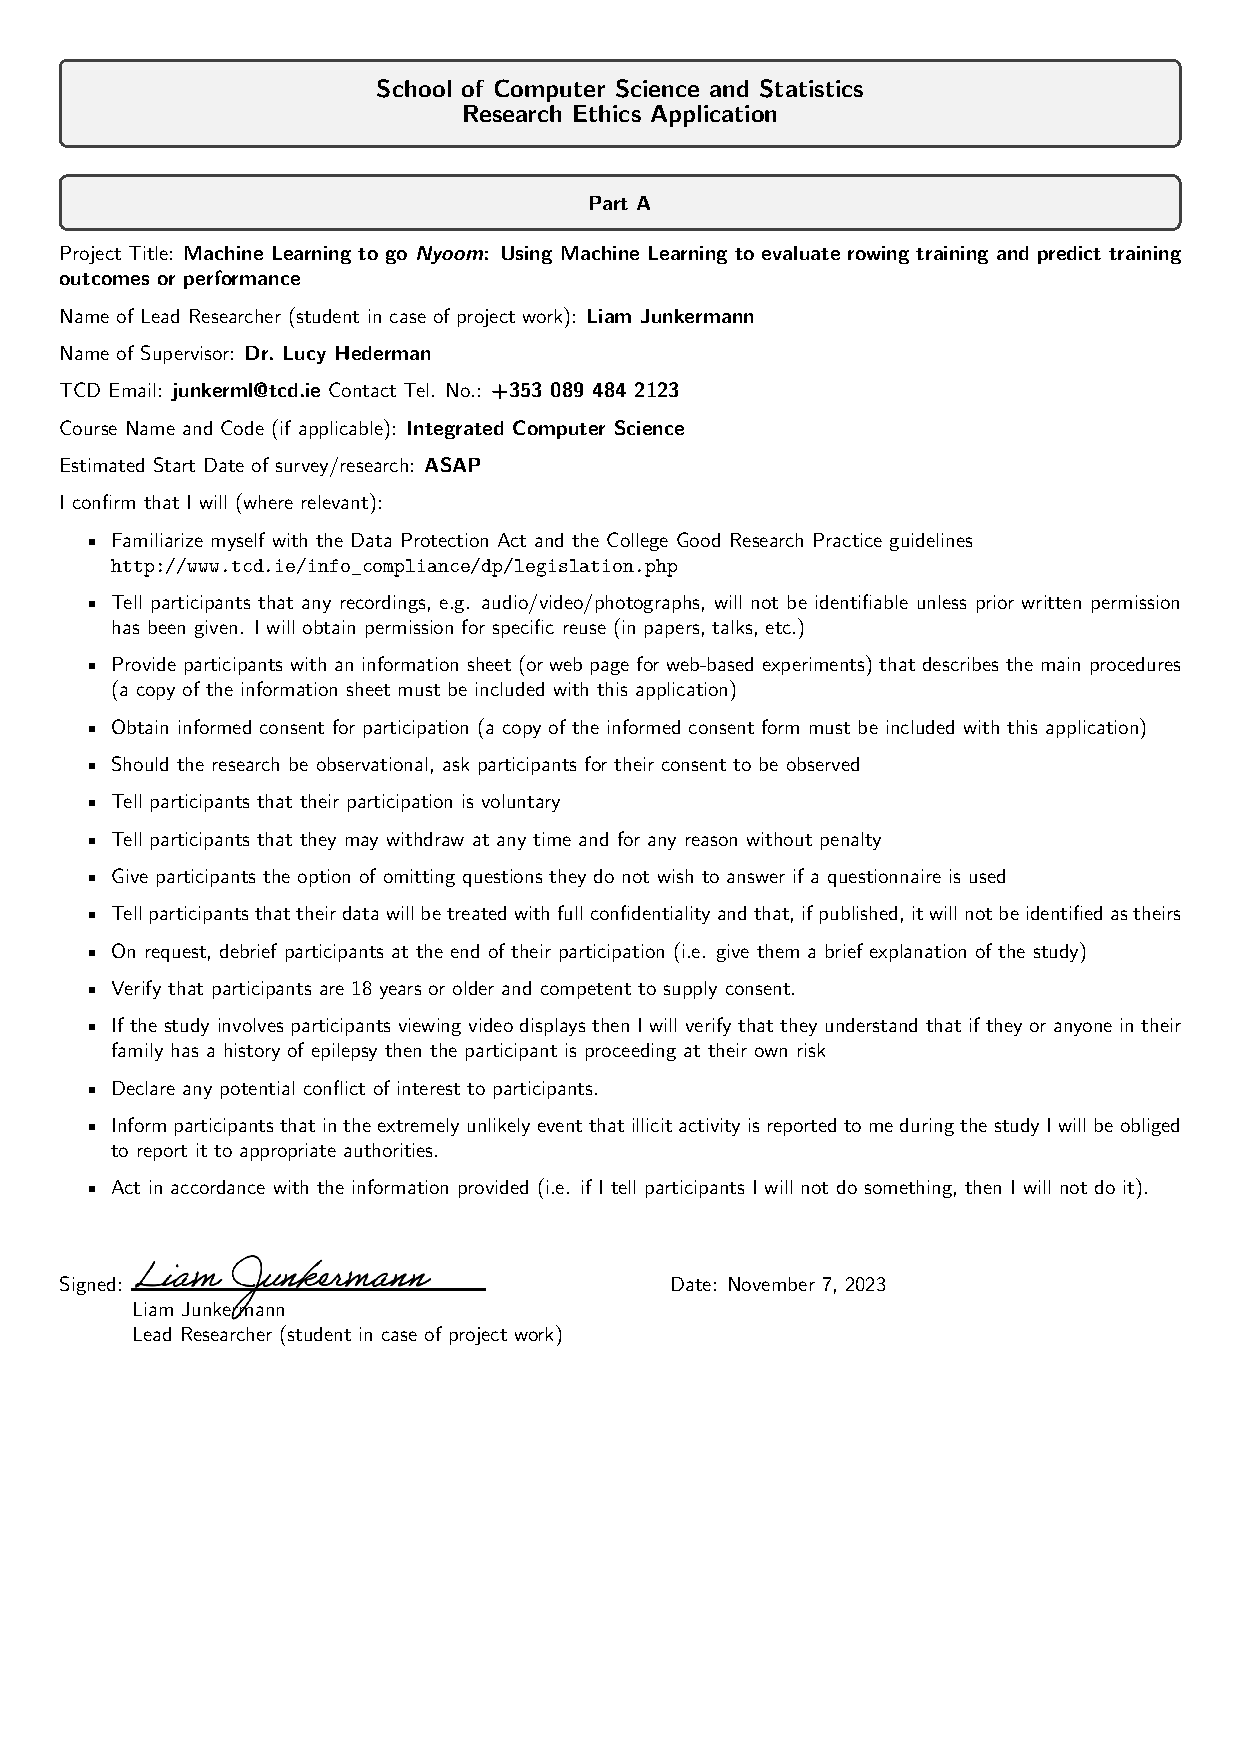
\includepdf[pages=-]{appendix/LiamJunkermannRevisedEthicsProposal_SignedLJLH.pdf}


\end{document}